\documentclass[12pt,a4paper]{report}

% ===================== NGÔN NGỮ & FONT =====================
\usepackage[utf8]{vietnam}
\usepackage{mathptmx}

% ===================== TRANG & BỐ CỤC =====================
\usepackage[a4paper,margin=2.5cm]{geometry}
\usepackage{setspace}
\setstretch{1.25}
\usepackage{titlesec}
\usepackage{fancyhdr}
\setlength{\headheight}{30pt}
\usepackage{enumitem}
\setlist[itemize]{label=-}
\setlist{topsep=4pt, itemsep=2pt}
\usepackage{float}

% ===================== TOÁN =====================
\usepackage{amsmath,amssymb,amsthm}

% ===================== HÌNH VẼ =====================
\usepackage{tikz}
\usetikzlibrary{calc,arrows.meta,positioning,patterns}
\usepackage{pgfplots}
\pgfplotsset{compat=1.18}
\usetikzlibrary{patterns.meta}

% ===================== BẢNG =====================
\usepackage{booktabs}
\usepackage{array}
\usepackage{capt-of}

% ===================== MÀU & HỘP NHẤN MẠNH =====================
\usepackage{xcolor}
\usepackage[most]{tcolorbox}

\usepackage{url}
% Mau chinh (dung cho tieu de chuong/muc, khung ngoai)
\definecolor{navy}{HTML}{1C2E58}
\definecolor{navylight}{HTML}{A9B8CE}
\definecolor{navybg}{HTML}{EEF1F6}

% Moi loai hop mot mau rieng, nen la ban nhat (8-10%) cua mau vien
\definecolor{teal}{HTML}{1F6F5C}      % Vi du
\definecolor{tealbg}{HTML}{E8F2EF}
\definecolor{plum}{HTML}{5B3A6E}      % Phuong phap
\definecolor{plumbg}{HTML}{F1EAF4}
\definecolor{burgundy}{HTML}{8C3B3B}  % Luu y
\definecolor{burgundybg}{HTML}{F8EBEA}
\definecolor{ochre}{HTML}{A8763E}     % Bai toan thuc te
\definecolor{ochrebg}{HTML}{F6EFE3}
\definecolor{inktext}{HTML}{4A4F57}   % Nhan xet (khong dung navy, tranh trung dinh nghia)
\definecolor{inkbg}{HTML}{F3F3F2}
\definecolor{commentgray}{HTML}{6E6E6E}
\definecolor{shadowgray}{HTML}{D7D7D7}
\definecolor{foldshade}{HTML}{E7EAF0}

\definecolor{linered}{HTML}{D62828}
\definecolor{linegreen}{HTML}{1B8A5A}
\definecolor{labelcolor}{HTML}{7B2CBF}

\newcommand{\bannerfont}{\sffamily}

% -- Các hộp: định nghĩa, ví dụ, nhận xét, lưu ý, phương pháp, ứng dụng --
\newtcolorbox{definitionbox}[1][]{%
  enhanced, breakable, colback=navybg, colframe=navy,
  boxrule=0.6pt, arc=2pt, left=6pt, right=6pt, top=4pt, bottom=4pt,
  fonttitle=\bannerfont\bfseries\color{white},
  colbacktitle=navy,
  title={Định nghĩa#1},
}
\newtcolorbox{examplebox}[1][]{%
  enhanced, breakable, colback=tealbg, colframe=teal,
  boxrule=0.6pt, arc=2pt, left=6pt, right=6pt, top=4pt, bottom=4pt,
  fonttitle=\bannerfont\bfseries\color{white},
  colbacktitle=teal,
  title={Ví dụ#1},
}
\newtcolorbox{notebox}[1][]{%
  enhanced, breakable, colback=inkbg, colframe=inktext!60,
  boxrule=0.5pt, arc=2pt, left=6pt, right=6pt, top=4pt, bottom=4pt,
  fonttitle=\bannerfont\bfseries\color{inktext},
  colbacktitle=inkbg,
  coltitle=inktext,
  title={Nhận xét#1},
}
\newtcolorbox{warningbox}[1][]{%
  enhanced, breakable, colback=burgundybg, colframe=burgundy,
  boxrule=0.8pt, arc=2pt, left=6pt, right=6pt, top=4pt, bottom=4pt,
  fonttitle=\bannerfont\bfseries\color{white},
  colbacktitle=burgundy,
  title={Lưu ý#1},
}
\newtcolorbox{methodbox}[1][]{%
  enhanced, breakable, colback=plumbg, colframe=plum,
  boxrule=0.6pt, arc=2pt, left=6pt, right=6pt, top=4pt, bottom=4pt,
  fonttitle=\bannerfont\bfseries\color{white},
  colbacktitle=plum,
  title={Phương pháp#1},
}
\newtcolorbox{applicationbox}[1][]{%
  enhanced, breakable, colback=ochrebg, colframe=ochre,
  boxrule=0.6pt, arc=2pt, left=6pt, right=6pt, top=4pt, bottom=4pt,
  fonttitle=\bannerfont\bfseries\color{white},
  colbacktitle=ochre,
  title={Bài toán thực tế#1},
}
\newenvironment{luuybox}{\begin{warningbox}}{\end{warningbox}}
\newtcolorbox{vidubox}[1][]{%
  enhanced, breakable, colback=tealbg, colframe=teal,
  boxrule=0.6pt, arc=2pt, left=6pt, right=6pt, top=4pt, bottom=4pt,
  fonttitle=\bannerfont\bfseries\color{white},
  colbacktitle=teal,
  title={#1},
}
\newtcolorbox{congthucbox}{%
  enhanced, breakable, colback=plumbg, colframe=plum,
  boxrule=0.6pt, arc=2pt, left=6pt, right=6pt, top=4pt, bottom=4pt,
  fonttitle=\bannerfont\bfseries\color{white},
  colbacktitle=plum,
  title={Quy trình gợi ý},
}

% ===================== TIÊU ĐỀ CHƯƠNG/MỤC =====================
\titleformat{\chapter}[display]
  {\bannerfont\Huge\bfseries\color{navy}}
  {\filright\Large\textcolor{navy}{CHƯƠNG \thechapter}}
  {6pt}
  {\filright}
\titleformat{\section}
  {\bannerfont\bfseries\Large\color{navy}}{\thesection}{8pt}{}
\titleformat{\subsection}
  {\bannerfont\bfseries\large\color{navy}}{\thesubsection}{6pt}{}
% ===================== HEADER/FOOTER =====================
\pagestyle{fancy}
\fancyhf{}
\renewcommand{\headrulewidth}{0.4pt}
\renewcommand{\footrulewidth}{0pt}
\fancyhead[L]{}
\fancyhead[R]{\small\textcolor{navy}{\leftmark}}
\fancyfoot[C]{\small\thepage}

% ===================== LIÊN KẾT NỘI BỘ =====================
\usepackage[colorlinks=true, linkcolor=navy, citecolor=navy, urlcolor=navy]{hyperref}
\tcbuselibrary{listings}

% 1. Khai báo style cơ bản cho code
\lstdefinestyle{pythonstyle}{
  language=Python,
  basicstyle=\ttfamily\small,
  keywordstyle=\color{violet!70!black}\bfseries,
  commentstyle=\color{black!50}\itshape,
  stringstyle=\color{teal!70!black},
  showstringspaces=false,
  breaklines=true,
  tabsize=2,
  % --- CÁC LỆNH HIỂN THỊ SỐ DÒNG ---
  numbers=left,                    % Bật số dòng ở bên trái
  numberstyle=\tiny\color{gray},   % Kích thước và màu sắc của số dòng
  numbersep=8pt,                   % Khoảng cách từ số dòng đến chữ
  xleftmargin=15pt                 % Đẩy lề mã lệnh sang phải 15pt để lấy chỗ chứa số
}

\lstdefinestyle{outputstyle}{
  basicstyle=\ttfamily\small\color{black},
  numbers=none,
  breaklines=true,
  showstringspaces=false,
}

% 2. Định nghĩa Tcolorbox chứa trực tiếp Listing
\newtcblisting{madoanbox}[1][Đoạn mã áp dụng]{%
  listing only, % Chỉ chứa code, không chứa văn bản LaTeX
  breakable, enhanced, colback=black!3, colframe=black!45,
  boxrule=0.5pt, arc=1mm, left=6pt, right=6pt, top=4pt, bottom=4pt,
  fonttitle=\sffamily\bfseries, coltitle=white,
  colbacktitle=black!55,
  title=#1,
  listing options={style=pythonstyle} % Gắn style python vào đây
}

\newtcblisting{ketquabox}[1][Kết quả chạy chương trình]{%
  listing only,
  breakable, enhanced, colback=gray!5, colframe=gray!55!black,
  boxrule=0.5pt, arc=1mm, left=6pt, right=6pt, top=4pt, bottom=4pt,
  fonttitle=\sffamily\bfseries, coltitle=white,
  colbacktitle=gray!55!black,
  title=#1,
  listing options={style=outputstyle} % Gắn style output vào đây
}

\begin{document}
\hypersetup{pageanchor=false}

% ============================================================================
%  TRANG BIA (Đã xóa hình, căn chỉnh bố cục tự động)
% ============================================================================
\newgeometry{left=2.8cm,right=2.8cm,top=2.6cm,bottom=2.4cm}
\begin{titlepage}
\centering

% --- Khung vien kep quanh trang ---
\begin{tikzpicture}[remember picture,overlay]
  \draw[navy,line width=2.2pt]
    ($(current page.north west)+(1.4cm,-1.4cm)$) rectangle
    ($(current page.south east)+(-1.4cm,1.4cm)$);
  \draw[navy,line width=0.6pt]
    ($(current page.north west)+(1.75cm,-1.75cm)$) rectangle
    ($(current page.south east)+(-1.75cm,1.75cm)$);
\end{tikzpicture}

% --- Tieu de co quan ---
{\large\bfseries ĐẠI HỌC HUẾ\par}
{\large\bfseries TRƯỜNG ĐẠI HỌC SƯ PHẠM\par}
\vspace{3pt}
{\large\bfseries KHOA TOÁN\par}
\vspace{6pt}
{\color{navy}\rule{4.2cm}{0.8pt}\par}

% Tăng nhẹ khoảng cách này để cụm tiêu đề rơi vào điểm nhìn đẹp nhất
\vspace{1.2cm}

{\Large\bfseries\color{navy} DỰ ÁN\par}
\vspace{0.4cm}
{\Large\bfseries\color{navy} ỨNG DỤNG SYMPY VÀO BÀI TOÁN\par}
\vspace{3pt}
{\Large\bfseries\color{navy} HỆ BẤT PHƯƠNG TRÌNH BẬC NHẤT HAI ẨN\par}

\vspace{0.8cm}

% --- Thong tin học phần ---
{\large\itshape Học phần: Tích hợp CNTT trong dạy Toán\par}

% Khoảng trống co giãn số 1: Tự động đẩy phần Bài làm nhóm xuống sao cho cân bằng
\vfill

% --- Thong tin nhom ---
{\large\bfseries BÀI LÀM NHÓM\par}
\vspace{6pt}
{\renewcommand{\arraystretch}{1.45}
\begin{tabular}{@{}l@{\hspace{1.2cm}}l@{}}
\toprule
\textbf{Họ và tên} & \textbf{Mã sinh viên} \\
\midrule
Dương Thế Tâm & 23S1010035 \\
Nguyễn Cao Minh Phúc & 23S1010027 \\
Ngô Hữu Trí & 23S1010045 \\
Trịnh Việt Anh Minh & 22S1010051 \\
\bottomrule
\end{tabular}\par}

\vspace{0.4cm}
\textbf{Giảng viên:} TS. Nguyễn Đăng Minh Phúc\par

% Khoảng trống co giãn số 2: Tự động đẩy dòng địa điểm, thời gian sát xuống lề dưới
\vfill
{\large Huế, 9/2026\par}
\vspace{0.3cm}

\end{titlepage}
\restoregeometry

\hypersetup{pageanchor=true}
\pagenumbering{roman}
% ============================================================
% LỜI CẢM ƠN
% ============================================================
\chapter*{Lời cảm ơn}
\addcontentsline{toc}{chapter}{Lời cảm ơn}

Trong quá trình thực hiện tiểu luận "Ứng dụng SymPy vào bài toán hệ bất phương trình bậc nhất hai ẩn", nhóm chúng em đã nhận được sự hướng dẫn tận tình từ thầy Nguyễn Đăng Minh Phúc. Những góp ý của thầy về cách tiếp cận nội dung toán học cũng như định hướng ứng dụng công cụ tính toán đã giúp nhóm hoàn thiện đề tài một cách rõ ràng và có hệ thống hơn.

Nhóm cũng xin gửi lời cảm ơn đến Khoa Toán và Trường Đại học Sư phạm, Đại học Huế, đã tạo điều kiện học tập và tài liệu tham khảo cần thiết trong suốt quá trình thực hiện tiểu luận này.

Do thời gian và kiến thức còn hạn chế, tiểu luận khó tránh khỏi những thiếu sót. Nhóm rất mong nhận được sự góp ý từ thầy để tiếp tục hoàn thiện.

\vspace{0.5cm}
\begin{flushright}
\textit{Huế, tháng 9 năm 2026}\\
\textit{Nhóm thực hiện}
\end{flushright}

\newpage

% ============================================================
% MỤC LỤC
% ============================================================
\tableofcontents
\newpage

% ============================================================
% MỞ ĐẦU
% ============================================================
\chapter*{Mở đầu}
\addcontentsline{toc}{chapter}{Mở đầu}

\section*{1. Lý do chọn đề tài}

Hệ bất phương trình bậc nhất hai ẩn là một trong những nội dung đầu tiên của chương trình Toán 10 đòi hỏi học sinh phối hợp đồng thời tư duy đại số và tư duy hình học \cite{sgk10-ktt}: một hệ vài bất phương trình trên giấy phải được chuyển thành một hình vẽ với nhiều đường thẳng, nhiều nửa mặt phẳng chồng lên nhau, rồi từ hình vẽ đó đọc lại miền nghiệm bằng lời. Với hệ chỉ hai hoặc ba bất phương trình, việc vẽ tay vẫn khả thi và chính là cách Chương~1 của tiểu luận này trình bày. Nhưng khi số bất phương trình tăng lên, số cặp đường biên cần xét giao điểm tăng theo tổ hợp, và việc loại bỏ bằng tay những giao điểm không thỏa mãn các bất phương trình còn lại trở thành một nguồn sai sót phổ biến, điều Chương~1 đã chỉ ra cụ thể ở mục các sai lầm thường gặp.

Song song đó, công cụ tính toán ký hiệu đã trở thành một phần quen thuộc của việc dạy và học toán ở nhiều nơi, không chỉ để tính nhanh mà còn để kiểm chứng lại một lập luận đã làm bằng tay. SymPy là một hệ đại số máy tính mã nguồn mở, viết bằng Python, đủ để giải hệ bất phương trình bằng ký hiệu; đi kèm với Matplotlib, một thư viện vẽ đồ họa hai chiều cũng của hệ sinh thái Python, hai công cụ này đủ để dựng một chương trình vừa giải được hệ bất phương trình, vừa vẽ lại miền nghiệm một cách chính xác. Vì cả hai đều miễn phí và chạy được trên một máy tính cá nhân thông thường, chúng phù hợp để một sinh viên hoặc giáo viên Toán tự xây dựng công cụ dạy học của riêng mình mà không phụ thuộc vào phần mềm thương mại.

Là sinh viên ngành Sư phạm Toán, nhóm chọn đề tài này vì nó đặt đúng vào điểm giao giữa hai việc cần làm song song trong quá trình đào tạo: nắm vững bản chất toán học của một nội dung sẽ trực tiếp giảng dạy sau này, và biết cách dùng công cụ tính toán để hỗ trợ việc dạy nội dung đó, thay vì xem công cụ như một hộp đen chỉ cho ra đáp số. Quá trình tự viết chương trình, như trình bày ở Chương~2 và áp dụng ở Chương~3, buộc nhóm phải hiểu rõ từng bước của phương pháp hình học đến mức có thể diễn đạt lại nó thành thuật toán, một cách kiểm tra sự hiểu bài nghiêm túc hơn nhiều so với việc chỉ giải lại các bài tập có sẵn.

\section*{2. Mục tiêu của tiểu luận}

Tiểu luận hướng tới các mục tiêu sau:
\begin{itemize}
\item Hệ thống hóa cơ sở toán học của bất phương trình và hệ bất phương trình bậc nhất hai ẩn, bao gồm khái niệm, biểu diễn hình học và phương pháp giải.
\item Tìm hiểu thư viện SymPy cùng các lệnh liên quan đến việc biểu diễn, xử lý biểu thức đại số và bất phương trình.
\item Xây dựng các ví dụ minh họa việc ứng dụng SymPy để giải và biểu diễn hệ bất phương trình bậc nhất hai ẩn, bao gồm cả các bài toán mô hình hóa thực tế.
\item Phân tích vai trò hỗ trợ của công cụ tính toán đối với việc học tập và dạy học nội dung này, đồng thời chỉ ra những giới hạn mà công cụ không thể thay thế tư duy toán học của người học.
\end{itemize}

\section*{3. Đối tượng nghiên cứu}

Đối tượng nghiên cứu của tiểu luận là các phương pháp biểu diễn và giải hệ bất phương trình bậc nhất hai ẩn, cùng với khả năng hỗ trợ của thư viện SymPy trong việc thực hiện các phương pháp đó.

\section*{4. Phạm vi nghiên cứu}

Tiểu luận giới hạn phạm vi nghiên cứu trong:
\begin{itemize}
\item Nội dung hệ bất phương trình bậc nhất hai ẩn thuộc chương trình Toán lớp 10;
\item Các chức năng của SymPy phù hợp và cần thiết cho nội dung nêu trên;
\item Không mở rộng sang các hệ bất phương trình phi tuyến hoặc các bài toán tối ưu tuyến tính phức tạp nằm ngoài phạm vi kiến thức phổ thông.
\end{itemize}

\section*{5. Phương pháp thực hiện}

Để thực hiện đề tài, nhóm sử dụng phối hợp các phương pháp sau: nghiên cứu tài liệu (sách giáo khoa, tài liệu hướng dẫn dạy học Toán, tài liệu chính thức của SymPy); phân tích nội dung toán học để xây dựng cơ sở lý thuyết ở Chương 1; thực nghiệm trên máy tính bằng SymPy; xây dựng và kiểm thử các ví dụ minh họa; và phân tích, so sánh kết quả giữa phương pháp giải thủ công và phương pháp sử dụng công cụ tính toán.

\section*{6. Cấu trúc tiểu luận}

Ngoài phần Mở đầu và Kết luận, nội dung chính của tiểu luận được trình bày trong ba chương:

\begin{itemize}
\item \textit{Chương 1} trình bày cơ sở toán học của hệ bất phương trình bậc nhất hai ẩn: khái niệm, biểu diễn hình học, phương pháp giải, các trường hợp đặc biệt của miền nghiệm, ứng dụng trong bài toán thực tế và những sai lầm thường gặp.
\item \textit{Chương 2} giới thiệu thư viện SymPy và các lệnh liên quan đến việc khai báo biến, biểu diễn biểu thức đại số và bất phương trình.
\item \textit{Chương 3} trình bày việc áp dụng chương trình của nhóm (mã nguồn đăng trên GitHub) vào các ví dụ cụ thể về hệ bất phương trình bậc nhất hai ẩn, đối chiếu với lời giải tay ở Chương~1, đồng thời đánh giá ưu điểm và hạn chế của chương trình.
\end{itemize}

\clearpage
\pagenumbering{arabic}

% ============================================================
% CHƯƠNG 1
% ============================================================
\chapter{HỆ BẤT PHƯƠNG TRÌNH BẬC NHẤT HAI ẨN}
\label{chap:hpt}

Trong chương trình Toán lớp 10, bài toán tìm tập hợp các điểm thỏa mãn một điều kiện tuyến tính là một trong những nội dung đầu tiên gắn kết chặt chẽ giữa đại số và hình học tọa độ. Chương này trình bày cơ sở toán học của bất phương trình và hệ bất phương trình bậc nhất hai ẩn, nền tảng cần thiết trước khi giới thiệu công cụ tính toán ở Chương 2 và áp dụng vào các bài toán cụ thể ở Chương 3.

\section{Khái quát về bất phương trình bậc nhất hai ẩn}
\label{sec:1.1}

\begin{definitionbox}
Bất phương trình bậc nhất hai ẩn $x,y$ là bất phương trình có một trong các dạng
\[
ax+by+c>0,\qquad ax+by+c<0,\qquad ax+by+c\ge 0,\qquad ax+by+c\le 0,
\]
trong đó $a,b,c\in\mathbb{R}$ cho trước, $a$ và $b$ không đồng thời bằng $0$.
\end{definitionbox}

Ở đây $x,y$ không đóng vai trò là hai đại lượng độc lập cần tìm riêng lẻ như trong phương trình một ẩn, mà được xem đồng thời như \textbf{tọa độ của một điểm} $M(x;y)$ trên mặt phẳng $Oxy$. Chính cách nhìn này tạo ra sự khác biệt căn bản so với bất phương trình một ẩn đã học: thay vì tập nghiệm là một khoảng trên trục số, tập nghiệm ở đây là một \emph{tập hợp điểm} trên mặt phẳng.

Một cặp số $(x_0;y_0)$ được gọi là \textbf{một nghiệm} của bất phương trình nếu khi thay $x=x_0,\ y=y_0$ vào, ta được một khẳng định đúng. Tập hợp tất cả các nghiệm như vậy được gọi là \textbf{tập nghiệm} của bất phương trình.

\begin{notebox}
Cần phân biệt rõ ba khái niệm thường bị nhầm lẫn: \textit{một nghiệm} là một cặp số cụ thể $(x_0;y_0)$; \textit{tập nghiệm} là toàn bộ (thường là vô số) các cặp số như vậy; \textit{biểu diễn hình học của tập nghiệm} là hình ảnh trực quan (một nửa mặt phẳng) thể hiện tập nghiệm đó trên hệ trục tọa độ, sẽ được trình bày ở mục~\ref{sec:1.2}.
\end{notebox}

\begin{examplebox}
Xét bất phương trình $2x-y+1>0$.

a) Với $(x_0;y_0)=(1;0)$: thay vào ta có $2\cdot 1-0+1=3>0$, đúng. Vậy $(1;0)$ là một nghiệm.

b) Với $(x_0;y_0)=(0;3)$: thay vào ta có $2\cdot 0-3+1=-2$, không thỏa $-2>0$. Vậy $(0;3)$ \emph{không} là nghiệm.

Có thể kiểm tra được rằng bất phương trình này có vô số nghiệm khác $(1;0)$, chẳng hạn $(2;0),\,(0;-2),\,(5;5),\dots$ Tập hợp tất cả các nghiệm đó tạo thành tập nghiệm của bất phương trình, và như sẽ thấy ngay sau đây, tập nghiệm này ứng với một nửa mặt phẳng.
\end{examplebox}

\section{Biểu diễn hình học của bất phương trình bậc nhất hai ẩn}
\label{sec:1.2}

Việc liệt kê từng nghiệm riêng lẻ như trên không cho ta hình dung tổng thể về tập nghiệm. Mục này xây dựng một cách biểu diễn hình học giúp \emph{nhìn thấy} toàn bộ tập nghiệm chỉ bằng một hình vẽ duy nhất.

\subsection{Đường thẳng biên}

\begin{definitionbox}[ (Đường biên)]
Xét bất phương trình $ax+by+c\ge 0$ (tương tự với $\le,\,>,\,<$). Đường thẳng
\[
d:\ ax+by+c=0
\]
được gọi là \textbf{đường biên} của bất phương trình. Đường thẳng $d$ chia mặt phẳng tọa độ $Oxy$ thành hai nửa mặt phẳng, và trên mỗi nửa mặt phẳng, biểu thức $ax+by+c$ giữ nguyên một dấu không đổi (luôn dương hoặc luôn âm).
\end{definitionbox}

Sở dĩ dấu của $ax+by+c$ không đổi trên mỗi nửa mặt phẳng là vì biểu thức này biến thiên liên tục theo $x,y$ và chỉ có thể triệt tiêu (bằng $0$) khi điểm $(x;y)$ nằm đúng trên đường biên $d$; do đó nó không thể "nhảy dấu" mà không đi qua $d$.

\begin{figure}[htbp]
\centering
\begin{tikzpicture}[scale=0.9]
\fill[navylight,opacity=0.3] (-2.5,-2) -- (2.5,2) -- (2.5,-2) -- cycle;
\fill[shadowgray,opacity=0.4] (-2.5,-2) -- (2.5,2) -- (-2.5,2) -- cycle;
\draw[-{Stealth[length=2mm]}] (-2.8,0) -- (2.9,0) node[right]{$x$};
\draw[-{Stealth[length=2mm]}] (0,-2.3) -- (0,2.3) node[above]{$y$};
\node[below left, font=\scriptsize] at (0,0) {$O$};
\draw[thick,navy] (-2.5,-2) -- (2.5,2) node[pos=0.85,above right, font=\scriptsize]{$d: ax+by+c=0$};
\node[navy, font=\scriptsize] at (1.6,-1) {$ax+by+c>0$};
\node[navy, font=\scriptsize] at (-1.6,1) {$ax+by+c<0$};
\end{tikzpicture}
\caption{Đường biên $d$ chia mặt phẳng thành hai nửa mặt phẳng, ứng với hai dấu của $ax+by+c$.}
\label{fig:duong-bien}
\end{figure}

\subsection{Cách xác định nửa mặt phẳng nghiệm}

\begin{methodbox}[ (dùng điểm thử)]
\begin{enumerate}
\item Vẽ đường thẳng biên $d: ax+by+c=0$.
\item Chọn một điểm $M(x_0;y_0)$ \emph{không} nằm trên $d$ (thường chọn $O(0;0)$ nếu $O\notin d$).
\item Thay tọa độ của $M$ vào biểu thức $ax+by+c$.
\item Nếu giá trị nhận được thỏa mãn bất phương trình đã cho thì nửa mặt phẳng chứa $M$ chính là miền nghiệm.
\item Nếu không thỏa mãn thì miền nghiệm là nửa mặt phẳng còn lại (không chứa $M$).
\end{enumerate}
\end{methodbox}

\begin{notebox}[ (quy ước vẽ đường biên)]
\begin{itemize}
\item Dấu $\ge$ hoặc $\le$: đường biên \textbf{thuộc} tập nghiệm $\Rightarrow$ vẽ bằng \textbf{nét liền}.
\item Dấu $>$ hoặc $<$: đường biên \textbf{không thuộc} tập nghiệm $\Rightarrow$ vẽ bằng \textbf{nét đứt}.
\end{itemize}
\end{notebox}

\begin{examplebox}[ 1]
Xác định và biểu diễn miền nghiệm của bất phương trình $x+y-2\ge 0$.

\emph{Đường biên:} $d: x+y-2=0$, đi qua $(2;0)$ và $(0;2)$.

\emph{Điểm thử:} chọn $O(0;0)\notin d$ (vì $0+0-2=-2\ne 0$). Thay vào vế trái: $-2$, không thỏa $-2\ge 0$.

\emph{Kết luận:} miền nghiệm là nửa mặt phẳng \emph{không} chứa $O$, kể cả đường biên (nét liền vì dấu $\ge$).
\end{examplebox}

\begin{figure}[H]
\centering
\begin{tikzpicture}[scale=0.85]
  \begin{scope}
    \clip (-1.2,-1.2) rectangle (3.2,3.2);
    \fill[pattern={Lines[angle=45,distance=5pt,line width=0.3pt]}, pattern color=navy]
      (-1.2,3.2) -- (3.2,-1.2) -- (-1.2,-1.2) -- cycle;
  \end{scope}
\draw[thick,navy] (-1.2,3.2) -- (3.2,-1.2)
  node[pos=0.9, sloped, above, font=\scriptsize]{$d:\ x+y-2=0$};
  \draw[-{Stealth[length=2mm]}] (-1.5,0) -- (3.6,0) node[right]{$x$};
  \draw[-{Stealth[length=2mm]}] (0,-1.5) -- (0,3.6) node[above]{$y$};
  \filldraw[navy] (0,0) circle (1.4pt);
  \node[below right, font=\scriptsize, fill=white, inner sep=0.5pt] at (0,0) {$O$};
  \node[navy, font=\scriptsize] at (2.1,2.1) {miền nghiệm};
\end{tikzpicture}
\caption{Miền nghiệm của bất phương trình $x+y-2\ge 0$ (kể cả đường biên); phần không phải nghiệm được gạch.}
\label{fig:vd-mien-nghiem-1}
\end{figure}

\begin{examplebox}[ 2]
Xác định miền nghiệm của bất phương trình $2x-y-1<0$.

\emph{Đường biên:} $d: 2x-y-1=0$, đi qua $(0;-1)$ và $(1;1)$.

\emph{Điểm thử:} chọn $O(0;0)$: $2\cdot 0-0-1=-1$, thỏa $-1<0$.

\emph{Kết luận:} miền nghiệm là nửa mặt phẳng \emph{chứa} $O$, \emph{không kể} đường biên (nét đứt vì dấu $<$ nghiêm ngặt).
\end{examplebox}

\section{Hệ bất phương trình bậc nhất hai ẩn}
\label{sec:1.3}

\subsection{Khái niệm hệ bất phương trình bậc nhất hai ẩn}

\begin{definitionbox}
Hệ bất phương trình bậc nhất hai ẩn là một hệ gồm từ hai bất phương trình bậc nhất hai ẩn $x,y$ trở lên, chẳng hạn
\[
\begin{cases}
a_1x+b_1y+c_1 \ge 0,\\
a_2x+b_2y+c_2 \ge 0,\\
\ \vdots
\end{cases}
\]
(các dấu $>,<,\ge,\le$ có thể phối hợp khác nhau giữa các bất phương trình trong hệ). Một cặp số $(x_0;y_0)$ được gọi là \textbf{một nghiệm} của hệ nếu nó đồng thời thỏa mãn \emph{tất cả} các bất phương trình trong hệ. Tập hợp tất cả các nghiệm như vậy gọi là \textbf{tập nghiệm của hệ}.
\end{definitionbox}

Điểm mấu chốt cần nắm là: nghiệm của hệ không phải nghiệm của riêng một bất phương trình nào, mà phải thỏa mãn \emph{đồng thời} mọi bất phương trình, do đó tập nghiệm của hệ chính là \textbf{giao} của các tập nghiệm thành phần.

\subsection{Biểu diễn hình học tập nghiệm của hệ}

Vì mỗi bất phương trình ứng với một nửa mặt phẳng, nên hệ bất phương trình ứng với phần giao của các nửa mặt phẳng đó.

\begin{figure}[htbp]
\centering
\begin{tikzpicture}[scale=0.85]
  \begin{scope}
    \clip (-1,-1.7) rectangle (3.2,2.7);
    \fill[pattern={Lines[angle=45,distance=5pt,line width=0.3pt]}, pattern color=navy]
      (-1,2.5) -- (3.2,-1.7) -- (-1,-1.7) -- cycle;
    \fill[pattern={Lines[angle=135,distance=5pt,line width=0.3pt]}, pattern color=navy!55]
      (-1,-1.5) -- (3.2,2.7) -- (-1,2.7) -- cycle;
  \end{scope}

  \draw[thick,navy]    (-1,2.5)  -- (3.2,-1.7) node[pos=0.92,sloped,  above, font=\scriptsize]{$d_1$};
  \draw[thick,navy!55] (-1,-1.5) -- (3.2,2.7)  node[pos=0.92,sloped, above, font=\scriptsize]{$d_2$};

  \draw[-{Stealth[length=2mm]}] (-1.3,0) -- (3.6,0) node[right]{$x$};
  \draw[-{Stealth[length=2mm]}] (0,-2)   -- (0,2.9) node[above]{$y$};

  \node[navy, font=\scriptsize, align=center] at (2.2,0.5) {miền nghiệm\\của hệ};
\end{tikzpicture}
\caption{Tập nghiệm của hệ hai bất phương trình là phần giao của hai nửa mặt phẳng tương ứng (phần không phải nghiệm được gạch).}
\label{fig:giao-hai-nua-mp}
\end{figure}

Tùy theo số lượng và vị trí tương đối của các đường biên, phần giao này có thể là một miền đa giác (bị chặn), một miền không bị chặn, một điểm duy nhất, hoặc tập rỗng (hệ vô nghiệm). Các trường hợp này được phân tích kèm ví dụ ở mục~\ref{sec:1.6}.

\section{Phương pháp giải hệ bất phương trình bậc nhất hai ẩn bằng phương pháp hình học}
\label{sec:1.4}

\begin{methodbox}[ (giải hệ bất phương trình bằng hình học)]
\textbf{Bước 1.} Đưa mỗi bất phương trình trong hệ về dạng $ax+by+c\ \Box\ 0$ (với $\Box\in\{>,<,\ge,\le\}$).\\
\textbf{Bước 2.} Với mỗi bất phương trình, xác định đường biên $d_i: a_ix+b_iy+c_i=0$.\\
\textbf{Bước 3.} Vẽ tất cả các đường biên $d_1,d_2,\dots$ trên cùng một hệ trục tọa độ $Oxy$.\\
\textbf{Bước 4.} Với mỗi đường biên, dùng điểm thử để xác định và tô miền nghiệm của riêng bất phương trình đó (mục~\ref{sec:1.2}).\\
\textbf{Bước 5.} Xác định phần mặt phẳng thuộc \emph{đồng thời} tất cả các miền nghiệm thành phần (phần không bị gạch/tô của bất kỳ bất phương trình nào).\\
\textbf{Bước 6.} Kết luận: phần mặt phẳng còn lại chính là miền nghiệm của hệ; nêu rõ hình dạng (đa giác, không bị chặn, một điểm,...) và các đỉnh nếu có.
\end{methodbox}

\begin{notebox}
Khi hệ có nhiều bất phương trình, các bước trên khó làm tay hơn: số cặp đường biên cần tìm giao điểm tăng nhanh, mỗi giao điểm phải được thay vào mọi bất phương trình còn lại để biết có phải đỉnh của miền nghiệm hay không, và hình vẽ tay có nhiều đường thẳng chồng lên nhau khó giữ chính xác. Chương~2 và Chương~3 dùng công cụ tính toán để hỗ trợ đúng những thao tác này.
\end{notebox}

\begin{examplebox}[ 1 (hệ hai bất phương trình, miền không bị chặn)]
\textbf{Đề bài.} Xác định miền nghiệm của hệ
\[
\begin{cases}
x-y\le 1,\\
x+y\ge -1.
\end{cases}
\]

\textbf{Các bước thực hiện.}
\begin{itemize}
\item $d_1: x-y=1$ đi qua $(1;0)$ và $(0;-1)$. Thử $O(0;0)$: $0-0=0\le 1$ đúng $\Rightarrow$ miền nghiệm của bpt 1 chứa $O$, biên nét liền.
\item $d_2: x+y=-1$ đi qua $(-1;0)$ và $(0;-1)$. Thử $O(0;0)$: $0+0=0\ge -1$ đúng $\Rightarrow$ miền nghiệm của bpt 2 chứa $O$, biên nét liền.
\item Hai đường biên cắt nhau tại điểm thỏa $x-y=1,\ x+y=-1$, giải ra $x=0,\ y=-1$, tức $A(0;-1)$.
\end{itemize}

\begin{center}
\begin{tikzpicture}[scale=0.8]
  \begin{scope}
    \clip (-3,-3) rectangle (3,3);
    \fill[pattern={Lines[angle=45,distance=5pt,line width=0.3pt]}, pattern color=navy]
      (-2,-3) -- (3,2) -- (3,-3) -- cycle;
    \fill[pattern={Lines[angle=135,distance=5pt,line width=0.3pt]}, pattern color=navy!55]
      (-3,2) -- (2,-3) -- (-3,-3) -- cycle;
  \end{scope}

  \draw[thick,navy]    (-2,-3) -- (3,2)
    node[pos=0.88, sloped, above, font=\scriptsize]{$d_1$};
  \draw[thick,navy!55] (-3,2)  -- (2,-3)
    node[pos=0.12, sloped, above, font=\scriptsize]{$d_2$};

  \draw[-{Stealth[length=2mm]}] (-3.3,0) -- (3.5,0) node[right]{$x$};
  \draw[-{Stealth[length=2mm]}] (0,-3.3) -- (0,3.4) node[above]{$y$};

  \filldraw[navy] (0,-1) circle (1.4pt);
  \node[right=2pt, font=\scriptsize, fill=white, inner sep=0.5pt] at (0,-1) {$A(0;-1)$};

  \node[navy, font=\scriptsize, align=center] at (1.1,1.9) {miền nghiệm\\của hệ};
\end{tikzpicture}
\captionof{figure}{Miền nghiệm của hệ ở Ví dụ 1 (phần không phải nghiệm được gạch).}
\label{fig:vd1-mien-nghiem}
\end{center}

\textbf{Kết luận.} Phần \textbf{để trắng} là miền nghiệm của hệ: một \emph{góc} không bị chặn, mở lên phía trên, với đỉnh $A(0;-1)$ và hai cạnh nằm trên $d_1$, $d_2$ (kể cả hai cạnh biên).
\end{examplebox}

\begin{examplebox}[ 2 (miền nghiệm là đa giác bị chặn)]
\textbf{Đề bài.} Xác định miền nghiệm của hệ
\[
\begin{cases}
x+y\le 4,\\
x\ge 0,\\
y\ge 0.
\end{cases}
\]

\textbf{Các bước thực hiện.}
\begin{itemize}
\item $x\ge 0,\ y\ge 0$: góc phần tư thứ nhất, đỉnh $O(0;0)$.
\item $d: x+y=4$ đi qua $(4;0)$ và $(0;4)$. Thử $O(0;0)$: $0+0=0\le 4$ đúng $\Rightarrow$ biên nét liền, miền nghiệm chứa $O$.
\item Tìm giao điểm từng cặp đường biên và kiểm tra thỏa các bất phương trình còn lại: $x=0$ và $y=0$ cho $O(0;0)$, thỏa $0+0\le4$, nhận; $x=0$ và $x+y=4$ cho $(0;4)$, thỏa $x\ge0$, nhận, gọi là $A$; $y=0$ và $x+y=4$ cho $(4;0)$, thỏa $y\ge0$, nhận, gọi là $B$.
\end{itemize}

\begin{center}
\begin{tikzpicture}[scale=0.85]
  \begin{scope}
    \clip (-1.5,-1.5) rectangle (5.5,5.5);
    \fill[pattern={Lines[angle=45,distance=5pt,line width=0.3pt]}, pattern color=navy]
      (-1.5,-1.5) rectangle (0,5.5);
    \fill[pattern={Lines[angle=135,distance=5pt,line width=0.3pt]}, pattern color=navy!55]
      (-1.5,-1.5) rectangle (5.5,0);
    \fill[pattern={Lines[angle=0,distance=5pt,line width=0.3pt]}, pattern color=navy!75]
      (-1.5,5.5) -- (5.5,-1.5) -- (5.5,5.5) -- cycle;
  \end{scope}

  \draw[thick,navy] (0,0) -- (4,0) -- (0,4) -- cycle;
  \draw[thick,navy] (-1.5,5.5) -- (5.5,-1.5)
    node[pos=0.5, sloped, below, font=\scriptsize]{$d: x+y=4$};

  \draw[-{Stealth[length=2mm]}] (-1.5,0) -- (5.8,0) node[right]{$x$};
  \draw[-{Stealth[length=2mm]}] (0,-1.5) -- (0,5.8) node[above]{$y$};

  \filldraw[navy] (0,0) circle (1.5pt);
  \node[below left, font=\scriptsize, fill=white, inner sep=0.5pt] at (0,0) {$O$};
  \filldraw[navy] (0,4) circle (1.5pt);
  \node[left=2pt, font=\scriptsize, fill=white, inner sep=0.5pt] at (0,4) {$A(0;4)$};
  \filldraw[navy] (4,0) circle (1.5pt);
  \node[below=2pt, font=\scriptsize, fill=white, inner sep=0.5pt] at (4,0) {$B(4;0)$};

  \node[navy, font=\scriptsize, align=center] at (1.25,1.25) {miền\\nghiệm};
\end{tikzpicture}
\captionof{figure}{Miền nghiệm của hệ ở Ví dụ 2 là tam giác $OAB$ (phần không phải nghiệm được gạch).}
\label{fig:vd3-tamgiac-tomtat}
\end{center}

\textbf{Kết luận.} Miền nghiệm là tam giác $OAB$ với $O(0;0),\,A(0;4),\,B(4;0)$, kể cả ba cạnh (vì cả ba bất phương trình đều có dấu $\ge,\le$ không nghiêm ngặt).

\textbf{Nhận xét.} Đây là dạng miền nghiệm thường gặp nhất trong các bài toán thực tế ở mục~\ref{sec:1.7}, khi các đại lượng $x,y$ (số sản phẩm, khối lượng,...) vừa bị chặn dưới bởi điều kiện không âm, vừa bị chặn trên bởi nguồn lực hữu hạn.
\end{examplebox}

\section{Một số trường hợp đặc biệt của miền nghiệm}
\label{sec:1.6}

\begin{enumerate}[label=(\arabic*)]
\item \textbf{Miền nghiệm bị chặn.} Xảy ra khi các nửa mặt phẳng "khép kín" lẫn nhau thành một đa giác hữu hạn, như tam giác $OAB$ ở Ví dụ 2 (mục~\ref{sec:1.4}).

\item \textbf{Miền nghiệm không bị chặn.} Xảy ra khi các nửa mặt phẳng không đủ để khép kín hoàn toàn, như ở Ví dụ 1 (mục~\ref{sec:1.4}), nơi miền nghiệm mở rộng vô hạn theo hai tia.

\item \textbf{Hệ vô nghiệm.} Xảy ra khi các nửa mặt phẳng không có điểm chung. Chẳng hạn với hệ
\[
\begin{cases}
x+y\le -1,\\
x+y\ge 1,
\end{cases}
\]
không tồn tại $(x;y)$ nào vừa có $x+y\le -1$ vừa có $x+y\ge 1$ (vì $-1<1$), nên hệ vô nghiệm.

\item \textbf{Miền nghiệm chỉ còn một điểm.} Xảy ra khi các điều kiện "siết chặt" lẫn nhau đến mức chỉ còn đúng một cặp $(x_0;y_0)$ thỏa mãn. Chẳng hạn với hệ
\[
\begin{cases}
x+y\ge 2,\\
x+y\le 2,\\
x\le 2,\\
y\le 0,
\end{cases}
\]
hai điều kiện đầu buộc $x+y=2$; kết hợp $y\le 0$ suy ra $x\ge 2$; kết hợp tiếp $x\le 2$ suy ra $x=2,\,y=0$. Vậy miền nghiệm chỉ gồm điểm duy nhất $(2;0)$.

\item \textbf{Miền nghiệm có/không chứa đường biên.} Như đã nêu ở mục~\ref{sec:1.2}, điều này phụ thuộc vào dấu của từng bất phương trình trong hệ ($\ge,\le$ thì chứa cạnh tương ứng; $>,<$ thì không). Với hệ nhiều bất phương trình, mỗi cạnh của đa giác nghiệm có thể chứa hoặc không chứa biên một cách \emph{độc lập} với các cạnh khác, tùy vào bất phương trình sinh ra cạnh đó, đây là điểm học sinh dễ nhầm lẫn nhất, sẽ được phân tích kỹ ở mục~\ref{sec:1.8}.
\end{enumerate}

\section{Ứng dụng hệ bất phương trình bậc nhất hai ẩn trong giải quyết vấn đề}
\label{sec:1.7}

Một trong những giá trị lớn nhất của hệ bất phương trình bậc nhất hai ẩn nằm ở khả năng \textbf{mô hình hóa} các tình huống thực tế có ràng buộc tuyến tính. Quy trình chuyển một bài toán thực tế thành hệ bất phương trình có thể tóm tắt như sau:

\[
\begin{aligned}
\text{Tình huống thực tế}
&\rightarrow \text{Xác định đại lượng}
\rightarrow \text{Đặt ẩn}
\rightarrow \text{Thiết lập điều kiện} \\
&\rightarrow \text{Lập hệ bất phương trình}
\rightarrow \text{Xác định miền nghiệm}
\rightarrow \text{Diễn giải kết quả}.
\end{aligned}
\]

\begin{warningbox}
Khi $x,y$ biểu diễn các đại lượng thực tế như số sản phẩm, số tiền, khối lượng,..., ngoài các bất phương trình phản ánh ràng buộc của đề bài, luôn cần bổ sung điều kiện \emph{không âm} $x\ge 0,\,y\ge 0$, và trong nhiều trường hợp còn cần điều kiện \emph{nguyên} $x,y\in\mathbb{Z}$. Do đó cần phân biệt \textbf{nghiệm toán học} (mọi điểm trong miền nghiệm) và \textbf{nghiệm có ý nghĩa thực tế} (chỉ những điểm thỏa thêm các điều kiện trên).
\end{warningbox}

\begin{applicationbox}[ : Bài toán sản xuất hai loại sản phẩm]
\textbf{Bối cảnh.} Một xưởng sản xuất hai loại sản phẩm $A$ và $B$. Nhu cầu về giờ máy, giờ nhân công và mức tối đa xưởng có mỗi ngày được cho trong bảng sau.

\begin{center}
\renewcommand{\arraystretch}{1.25}
\begin{tabular}{|l|c|c|c|}
\hline
 & \textbf{Sản phẩm $A$} & \textbf{Sản phẩm $B$} & \textbf{Tối đa mỗi ngày} \\
\hline
Giờ máy & $2$ & $1$ & $8$ \\
\hline
Giờ nhân công & $1$ & $3$ & $9$ \\
\hline
\end{tabular}
\end{center}

\textbf{Xác định biến.} Gọi $x$ là số sản phẩm loại $A$, $y$ là số sản phẩm loại $B$ sản xuất trong ngày ($x,y\ge 0$).

\textbf{Phân tích dữ kiện.} Tổng giờ máy sử dụng là $2x+y$, không vượt quá $8$. Tổng giờ nhân công sử dụng là $x+3y$, không vượt quá $9$.

\textbf{Lập hệ bất phương trình.}
\[
\begin{cases}
2x+y\le 8,\\
x+3y\le 9,\\
x\ge 0,\ y\ge 0.
\end{cases}
\]

\textbf{Biểu diễn miền nghiệm.} $d_1: 2x+y=8$ đi qua $(4;0)$ và $(0;8)$. Thử $O(0;0)$: $0\le 8$ đúng $\Rightarrow$ lấy nửa mặt phẳng chứa $O$. $d_2: x+3y=9$ đi qua $(9;0)$ và $(0;3)$. Thử $O(0;0)$: $0\le 9$ đúng $\Rightarrow$ lấy nửa mặt phẳng chứa $O$. Giao điểm của $d_1$ và $d_2$: giải hệ $2x+y=8,\ x+3y=9$ được $x=3,\ y=2$, tức $B(3;2)$. Các đỉnh còn lại: $O(0;0)$, $A(4;0)$ (giao của $d_1$ với $Ox$), $C(0;3)$ (giao của $d_2$ với $Oy$).

\begin{center}
\begin{tikzpicture}[scale=0.95]
  \begin{scope}
    \clip (-1,-1) rectangle (5.5,4.5);
    \fill[pattern={Lines[angle=90,distance=5pt,line width=0.3pt]}, pattern color=navy!35]
      (-1,-1) rectangle (0,4.5);
    \fill[pattern={Lines[angle=0,distance=5pt,line width=0.3pt]}, pattern color=navy!80]
      (-1,-1) rectangle (5.5,0);
    \fill[pattern={Lines[angle=45,distance=5pt,line width=0.3pt]}, pattern color=linered]
      (0,8) -- (4.5,-1) -- (5.5,-1) -- (5.5,8) -- cycle;
    \fill[pattern={Lines[angle=135,distance=5pt,line width=0.3pt]}, pattern color=linegreen]
      (-1,{10/3}) -- (5.5,{7/6}) -- (5.5,4.5) -- (-1,4.5) -- cycle;
  \end{scope}

  \draw[very thick,navy] (4,0) -- (0,0) -- (0,3);

  \draw[very thick,linered] (1.75,4.5) -- (4.5,-1)
    node[pos=0, above, font=\scriptsize\bfseries]{$d_1: 2x+y=8$};
  \draw[very thick,linegreen] (-1,{10/3}) -- (5.5,{7/6})
    node[pos=1, right, font=\scriptsize\bfseries]{$d_2: x+3y=9$};

  \foreach \i in {0,...,4}{
    \foreach \j in {0,...,3}{
      \pgfmathtruncatemacro{\ca}{2*\i+\j}
      \pgfmathtruncatemacro{\cb}{\i+3*\j}
      \ifnum\ca>8\else\ifnum\cb>9\else
        \fill[navy] (\i,\j) circle (1pt);
      \fi\fi
    }
  }

  \draw[-{Stealth[length=2mm]}] (-1,0) -- (5.8,0) node[right]{$x$};
  \draw[-{Stealth[length=2mm]}] (0,-1) -- (0,4.8) node[above]{$y$};

  \foreach \p in {(0,0),(4,0),(3,2),(0,3)}{\filldraw[navy] \p circle (1.6pt);}
  \node[below left,  font=\scriptsize\bfseries, text=labelcolor] at (0,0) {$O$};
  \node[below right, font=\scriptsize\bfseries, text=labelcolor] at (4,0) {$A(4;0)$};
  \node[right=2pt,   font=\scriptsize\bfseries, text=labelcolor] at (3,2.3) {$B(3;2)$};
  \node[left=2pt,    font=\scriptsize\bfseries, text=labelcolor] at (0,3) {$C(0;3)$};

  \node[font=\scriptsize\bfseries, text=labelcolor, align=center] at (1.3,1.1) {miền\\nghiệm};
\end{tikzpicture}
\captionof{figure}{Miền nghiệm của hệ là tứ giác $OABC$; các chấm nhỏ là điểm nguyên thuộc miền nghiệm.}
\label{fig:ud1-sanxuat}
\end{center}

\textbf{Diễn giải kết quả.} Miền nghiệm là tứ giác $OABC$ với $O(0;0)$, $A(4;0)$, $B(3;2)$, $C(0;3)$; mỗi điểm của tứ giác là một phương án sản xuất \emph{khả thi} về mặt toán học. Vì $x,y$ là số sản phẩm nên chỉ các điểm nguyên không âm trong tứ giác mới có ý nghĩa thực tế, chẳng hạn $B(3;2)$ hay $(2;1)$; điểm $B(3;2)$ nằm trên cả hai đường biên nên là phương án dùng hết cả giờ máy lẫn giờ nhân công, trong khi một điểm như $(2{,}5;1{,}5)$ tuy thuộc miền nghiệm toán học (vì $2\cdot 2{,}5+1{,}5=6{,}5\le 8$ và $2{,}5+3\cdot 1{,}5=7\le 9$) nhưng không có ý nghĩa sản xuất.
\end{applicationbox}

\section{Một số sai lầm của học sinh khi giải hệ bất phương trình hai ẩn}
\label{sec:1.8}

\begin{enumerate}[label=\textbf{(\arabic*)}, leftmargin=1.6cm]

\item \textbf{Nhầm bất phương trình với phương trình.}\\
\textit{Nguyên nhân:} thói quen từ việc giải phương trình khiến học sinh tìm "nghiệm duy nhất" thay vì miền nghiệm.\\
\textit{Ví dụ:} với $x+y\le 4$, học sinh chỉ giải $x+y=4$ rồi dừng lại, không xét đến cả một nửa mặt phẳng.\\
\textit{Khắc phục:} nhấn mạnh ngay từ đầu rằng nghiệm là \emph{tập hợp điểm}, và phương trình chỉ cho đường biên.

\item \textbf{Nhầm dấu $>,<$ với $\ge,\le$ khi vẽ hình.}\\
\textit{Nguyên nhân:} không chú ý đề bài, hoặc chép sai đề khi vẽ hình.\\
\textit{Ví dụ:} vẽ đường biên nét liền cho bất phương trình có dấu $<$ nghiêm ngặt.\\
\textit{Khắc phục:} luôn đối chiếu dấu của bất phương trình với quy ước nét liền/nét đứt trước khi vẽ.

\item \textbf{Chọn sai nửa mặt phẳng nghiệm hoặc bỏ qua bước thử điểm.}\\
\textit{Nguyên nhân:} học sinh "đoán" miền nghiệm dựa trên trực giác về dấu của $a,b$ mà không thử lại bằng số cụ thể (chẳng hạn cho rằng $ax+by+c\ge0$ luôn ứng với miền "phía trên" đường biên, điều này không đúng khi $b<0$), hoặc chọn điểm thử nằm ngay trên đường biên nên không xác định được dấu.\\
\textit{Ví dụ:} với $x+y-2\ge0$, học sinh chọn điểm thử $(2;0)$ (nằm trên đường biên) nên không xác định được dấu.\\
\textit{Khắc phục:} luôn kiểm tra điểm thử không thuộc đường biên trước khi thay vào, và luôn thực hiện đủ bước thay số, không suy luận cảm tính.

\item \textbf{Không lấy giao các miền nghiệm.}\\
\textit{Nguyên nhân:} với hệ nhiều bất phương trình, học sinh chỉ tô riêng lẻ từng miền mà không xác định phần chung.\\
\textit{Ví dụ:} tô đúng ba miền nghiệm riêng lẻ của ba bất phương trình nhưng kết luận nhầm miền nghiệm của hệ là hợp thay vì giao.\\
\textit{Khắc phục:} sau khi tô riêng, luôn xác định lại phần \emph{không} bị gạch bởi bất kỳ bất phương trình nào, đó mới là miền nghiệm của hệ.

\item \textbf{Không xét điều kiện thực tế của biến.}\\
\textit{Nguyên nhân:} khi giải bài toán mô hình hóa, học sinh dừng lại ở miền nghiệm toán học mà quên các ràng buộc $x,y\ge0$ hoặc $x,y\in\mathbb{Z}$.\\
\textit{Ví dụ:} kết luận "có thể sản xuất $3.5$ sản phẩm" trong bài toán sản xuất ở mục~\ref{sec:1.7}.\\
\textit{Khắc phục:} luôn đối chiếu lại nghiệm toán học với ý nghĩa thực tế của đề bài trước khi kết luận.
\item \textbf{Vẽ mọi đường biên cùng một kiểu nét.}\\
\textit{Nguyên nhân:} với hệ vừa có dấu chặt vừa có dấu không chặt, học sinh coi cả miền nghiệm là "có biên" hoặc "không biên" thay vì xét từng bất phương trình.\\
\textit{Ví dụ:} với hệ $x+y\le 4,\ x>0,\ y\ge 0$, học sinh vẽ cả ba cạnh của tam giác bằng nét liền, trong khi cạnh nằm trên $Oy$ (ứng với $x>0$) không thuộc miền nghiệm.\\
\textit{Khắc phục:} chọn kiểu nét cho từng đường biên theo bất phương trình sinh ra nó, rồi mới ghép các cạnh lại.

\end{enumerate}



\section{Tiểu kết chương 1}
\label{sec:1.10}

Chương này đã trình bày một cách hệ thống cơ sở toán học của bất phương trình và hệ bất phương trình bậc nhất hai ẩn. Xuất phát từ khái niệm bất phương trình bậc nhất hai ẩn và nghiệm của nó như một cặp số $(x_0;y_0)$, chương đã xây dựng biểu diễn hình học tương ứng: mỗi bất phương trình ứng với một nửa mặt phẳng, được xác định thông qua đường biên và phương pháp điểm thử, với quy ước nét liền/nét đứt phản ánh việc đường biên có thuộc miền nghiệm hay không.

Trên nền tảng đó, hệ bất phương trình bậc nhất hai ẩn được định nghĩa là sự kết hợp của nhiều bất phương trình, với tập nghiệm chính là giao của các nửa mặt phẳng thành phần. Phương pháp giải hình học được trình bày thành một quy trình sáu bước rõ ràng, minh họa qua hai ví dụ tăng dần độ khó, từ hệ hai bất phương trình cho miền không bị chặn, đến hệ ba bất phương trình cho miền đa giác bị chặn. Chương cũng đã phân loại các trường hợp đặc biệt của miền nghiệm: bị chặn, không bị chặn, vô nghiệm, hay chỉ gồm một điểm.

Chương đã chỉ ra khả năng ứng dụng của công cụ này trong việc mô hình hóa bài toán thực tế có ràng buộc tuyến tính, đồng thời phân tích những sai lầm phổ biến mà người học thường gặp phải, phần lớn xuất phát từ việc thực hiện thiếu một bước trong quy trình giải, hoặc từ sai sót khi vẽ hình bằng tay.

Chính những hạn chế mang tính kỹ thuật đó, tính tọa độ đỉnh thủ công, vẽ hình thiếu chính xác, khó kiểm soát khi số lượng bất phương trình tăng lên, tạo ra nhu cầu tự nhiên đối với một công cụ tính toán hỗ trợ đáng tin cậy. Từ cơ sở toán học vững chắc được xây dựng ở Chương~1, Chương~2 sẽ giới thiệu thư viện SymPy cùng các lệnh liên quan đến việc biểu diễn và xử lý biểu thức đại số, làm tiền đề để Chương~3 áp dụng cụ thể vào việc giải và biểu diễn hệ bất phương trình bậc nhất hai ẩn một cách tự động và chính xác.

\begin{thebibliography}{9}
\addcontentsline{toc}{chapter}{Tài liệu tham khảo}

\bibitem{sgk10-ktt}
Sách giáo khoa Toán 10, bộ \emph{Kết nối tri thức với cuộc sống}, Nhà xuất bản Giáo dục Việt Nam. \emph{(Nhóm bổ sung tên tác giả, năm xuất bản, ISBN cụ thể theo ấn bản đang sử dụng.)}

\bibitem{sbt10-ktt}
Sách bài tập Toán 10, bộ \emph{Kết nối tri thức với cuộc sống}, Nhà xuất bản Giáo dục Việt Nam. \emph{(Nhóm bổ sung tên tác giả, năm xuất bản, ISBN cụ thể theo ấn bản đang sử dụng.)}

\bibitem{sgv10-ktt}
Sách giáo viên Toán 10, bộ \emph{Kết nối tri thức với cuộc sống}, Nhà xuất bản Giáo dục Việt Nam. \emph{(Nhóm bổ sung thông tin xuất bản cụ thể.)}

\bibitem{tlhdgv}
Tài liệu hướng dẫn dạy học môn Toán cấp trung học phổ thông (tài liệu bồi dưỡng giáo viên), phần liên quan đến dạy học biểu diễn đại số và hình học, mô hình hóa toán học. \emph{(Nhóm bổ sung tên đơn vị biên soạn, năm phát hành cụ thể.)}

\end{thebibliography}

% ============================================================
% CHƯƠNG 2
% ============================================================
\chapter{GIỚI THIỆU SYMPY VÀ CÁC LỆNH LIÊN QUAN}
\label{chap:sympy}

Chương 1 đã xây dựng cơ sở toán học cho hệ bất phương trình bậc nhất hai ẩn và nêu ở mục~\ref{sec:1.4} những khó khăn khi giải bằng tay: tính tọa độ đỉnh thủ công, vẽ hình thiếu chính xác, dễ nhầm lẫn khi số lượng bất phương trình tăng lên.

Mỗi lệnh được trình bày theo bốn ý: lệnh làm gì, ý nghĩa toán học của nó, một ví dụ nhỏ và kết quả thu được. Các ví dụ ở chương này cố ý dùng những biểu thức đơn giản, tách khỏi chương trình chính, để người đọc tập trung vào bản thân lệnh. Chương trình hoàn chỉnh của nhóm ghép các lệnh này lại với nhau; mã nguồn được đăng trên GitHub, và Chương 3 áp dụng chương trình vào các ví dụ cụ thể.

\begin{table}[htbp]
\centering
\small
\begin{tabular}{@{}p{6.4cm}p{5.6cm}p{1.6cm}@{}}
\toprule
Thao tác toán học ở Chương 1 & Nhóm lệnh & Mục \\
\midrule
Khai báo hai ẩn $x,y$ & \texttt{symbols} & \ref{sec:2.3} \\
Chuyển vế, khai triển, rút gọn & \texttt{expand}, \texttt{factor}, \texttt{simplify} & \ref{sec:2.4} \\
Đọc một bất phương trình nhập dưới dạng chuỗi & \texttt{sympify} & \ref{sec:2.5} \\
Nhận biết dấu và hai vế của bất phương trình & \texttt{Eq}, \texttt{rel\_op}, \texttt{lhs}, \texttt{rhs} & \ref{sec:2.6} \\
Đưa về dạng $ax+by=c$ và đọc hệ số & \texttt{coeff}, \texttt{subs} & \ref{sec:2.7} \\
Thay tọa độ điểm để kiểm tra & \texttt{subs} & \ref{sec:2.8} \\
Tìm giao điểm hai đường biên & \texttt{solve}, \texttt{linsolve} & \ref{sec:2.9} \\
Tính toán số lặp lại và vẽ hình & NumPy, \texttt{itertools}, Matplotlib & \ref{sec:2.10} \\
\bottomrule
\end{tabular}
\caption{Đối chiếu thao tác toán học ở Chương 1 với nhóm lệnh được giới thiệu ở Chương 2.}
\label{tab:ban-do-lenh}
\end{table}

\section{Giới thiệu về SymPy}
\label{sec:2.1}

SymPy là một thư viện của ngôn ngữ Python dùng cho tính toán đại số ký hiệu (\textit{symbolic computation}). Điểm khác biệt cốt lõi so với tính toán số thông thường là SymPy làm việc trực tiếp trên biểu thức và giữ nguyên dạng chính xác của chúng, thay vì chuyển sang số thập phân gần đúng:

\begin{madoanbox}
import math
import sympy as sp

print(math.sqrt(8))
print(sp.sqrt(8))
\end{madoanbox}

\begin{ketquabox}
2.8284271247461903
2*sqrt(2)
\end{ketquabox}

Hàm \texttt{math.sqrt} trả về một giá trị gần đúng của $\sqrt{8}$, còn \texttt{sp.sqrt} trả về đúng biểu thức $2\sqrt{2}$, tức là kết quả rút gọn chính xác mà người học sẽ viết trên giấy.

SymPy là phần mềm mã nguồn mở, miễn phí, do cộng đồng phát triển và duy trì. Thư viện có thể khai triển và rút gọn biểu thức, giải phương trình và hệ phương trình, tính đạo hàm, tích phân, và nhiều thao tác đại số khác. Trong học tập Toán, SymPy có thể đóng vai trò một công cụ kiểm chứng: người học tự giải bài toán bằng phương pháp truyền thống, sau đó dùng SymPy đối chiếu để phát hiện sai sót trong tính toán.

Trong tiểu luận này, vai trò của SymPy được giới hạn rõ ràng: đọc và xử lý biểu thức, cụ thể là biến một bất phương trình được nhập dưới dạng chuỗi ký tự thành các hệ số $a,b,c$. Phần tính toán số lặp lại nhiều lần và phần vẽ hình do NumPy và Matplotlib đảm nhiệm.Sự phân công này được tóm tắt ở mục~\ref{sec:2.10}.

\section{Cài đặt và môi trường sử dụng}
\label{sec:2.2}

SymPy chạy trên nền Python, nên cần cài Python 3 (nên dùng phiên bản còn được hỗ trợ) trước. Sau đó cài SymPy, cùng NumPy và Matplotlib mà chương trình ở Chương 3 cần, bằng một lệnh trong terminal hoặc command prompt:

\begin{madoanbox}
pip install sympy numpy matplotlib
\end{madoanbox}

Để kiểm tra SymPy đã cài thành công và biết phiên bản đang dùng:

\begin{madoanbox}
import sympy
print(sympy.__version__)
\end{madoanbox}

Kết quả phụ thuộc vào phiên bản đã cài, chẳng hạn:

\begin{ketquabox}
1.14.0
\end{ketquabox}

Có nhiều môi trường để chạy các đoạn code này, mỗi môi trường phù hợp với một mục đích khác nhau:

\begin{itemize}
\item Jupyter Notebook: vừa viết code vừa xem kết quả ngay bên dưới, công thức toán được hiển thị trực quan, thuận tiện cho việc thử nghiệm và viết báo cáo.
\item Google Colab: tương tự Jupyter Notebook nhưng chạy trực tuyến, không cần cài đặt trên máy cá nhân, và thường đã có sẵn SymPy, NumPy, Matplotlib.
\item VS Code: phù hợp khi cần viết một chương trình hoàn chỉnh lưu thành tệp \texttt{.py}, như chương trình ở Chương 3.
\end{itemize}

\section{Khai báo biến}
\label{sec:2.3}

\textit{Lệnh.} Trước hết cần nhập thư viện và khai báo các ẩn:

\begin{madoanbox}
import sympy as sp

x, y = sp.symbols('x y', real=True)
print(x + y)
print(x.is_real)
\end{madoanbox}

\begin{ketquabox}
x + y
True
\end{ketquabox}

Dòng import đầu tiên nạp SymPy với bí danh \texttt{sp}. Nhờ bí danh này, các hàm được gọi ngắn gọn, chẳng hạn \texttt{sp.symbols}; đây là quy ước phổ biến trong cộng đồng Python. Lệnh tiếp theo tạo cùng lúc hai biến ký hiệu $x$ và $y$, với tên biến được ngăn cách bằng dấu cách. Khác với biến lập trình thông thường phải mang một giá trị cụ thể, biến ký hiệu đại diện cho một ẩn số toán học; vì vậy biểu thức \texttt{x + y} có thể tồn tại mà chưa cần gán giá trị.

\textit{Ý nghĩa toán học.} Hai biến này chính là hai ẩn $(x;y)$, tọa độ của một điểm trên mặt phẳng $Oxy$ như đã dùng xuyên suốt Chương 1. Tham số \texttt{real=True} khai báo rằng chúng chỉ nhận giá trị thực, đúng với bản chất của tọa độ. Đây không chỉ là chi tiết hình thức, vì nó ảnh hưởng đến kết quả rút gọn:

\begin{madoanbox}
u = sp.Symbol('u')
v = sp.Symbol('v', real=True)
print(sp.sqrt(u**2))
print(sp.sqrt(v**2))
\end{madoanbox}

\begin{ketquabox}
sqrt(u**2)
Abs(v)
\end{ketquabox}

Với $v$ thực, căn bậc hai của $v^2$ bằng $|v|$ nên SymPy rút gọn được. Với $u$ chưa biết thuộc tập số nào, đẳng thức đó không còn luôn đúng nên biểu thức được giữ nguyên.

Ngoài \texttt{real=True}, SymPy còn cho phép khai báo các ràng buộc khác như \texttt{positive=True} (dương), \texttt{nonnegative=True} (không âm), \texttt{integer=True} (nguyên). Các ràng buộc này tương ứng với điều kiện của biến trong bài toán thực tế ở mục~\ref*{sec:1.7}, Chương 1, nơi số sản phẩm phải không âm và là số nguyên:

\begin{madoanbox}
n = sp.symbols('n', integer=True, nonnegative=True)
print(n.is_integer, n.is_nonnegative)
\end{madoanbox}

\begin{ketquabox}
True True
\end{ketquabox}

\section{Biểu thức đại số}
\label{sec:2.4}

Sau khi có biến ký hiệu, ta viết các biểu thức đại số gần như cách viết trên giấy, với hai lưu ý về cú pháp: phép nhân được viết rõ bằng dấu \texttt{*} và lũy thừa được viết bằng \texttt{**}. Ba lệnh biến đổi cơ bản nhất là:

\begin{itemize}
\item \texttt{sp.expand(bt)}: khai triển biểu thức, tức phá ngoặc và đưa về tổng các đơn thức;
\item \texttt{sp.factor(bt)}: phân tích biểu thức thành nhân tử;
\item \texttt{sp.simplify(bt)}: rút gọn biểu thức về dạng đơn giản hơn.
\end{itemize}

\begin{madoanbox}
print(sp.expand((x + y)**2))
print(sp.factor(x**2 - y**2))
print(sp.simplify((x**2 - y**2)/(x - y)))
\end{madoanbox}

\begin{ketquabox}
x**2 + 2*x*y + y**2
(x - y)*(x + y)
x + y
\end{ketquabox}

\textit{Ý nghĩa toán học.} Ba kết quả trên là các hằng đẳng thức quen thuộc: $(x+y)^2=x^2+2xy+y^2$ và $x^2-y^2=(x-y)(x+y)$. Ở lệnh thứ ba, việc rút gọn phân thức thành $x+y$ đúng khi $x\ne y$, đúng như cách rút gọn trên giấy.

\begin{notebox}
Trong bài toán hệ bất phương trình bậc nhất hai ẩn, lệnh \texttt{expand} giữ vai trò chuẩn hóa: đưa vế trái của một bất phương trình về dạng tổng các đơn thức để có thể đọc đúng hệ số của $x$ và $y$. Vai trò này được minh họa cụ thể ở mục~\ref{sec:2.7}.
\end{notebox}

\section{Đọc biểu thức từ chuỗi}
\label{sec:2.5}

\textit{Lệnh.} Chương trình ở Chương 3 nhận các bất phương trình dưới dạng chuỗi ký tự, chẳng hạn \texttt{"x + y <= 2"}. Lệnh \texttt{sp.sympify} chuyển một chuỗi như vậy thành đối tượng toán học mà SymPy xử lý được:

\begin{madoanbox}
import sympy as sp
x, y = sp.symbols('x y', real=True)

bt = sp.sympify("2*x - y + 1", locals={'x': x, 'y': y})
print(bt)
print(type(bt))

bpt = sp.sympify("x + y <= 2", locals={'x': x, 'y': y})
print(bpt)
print(type(bpt))
\end{madoanbox}

\begin{ketquabox}
2*x - y + 1
<class 'sympy.core.add.Add'>
x + y <= 2
<class 'sympy.core.relational.LessThan'>
\end{ketquabox}

\textit{Ý nghĩa toán học.} Với máy tính, \texttt{"x + y <= 2"} ban đầu chỉ là một dãy ký tự, chưa mang nghĩa toán học nào. Sau \texttt{sympify}, nó trở thành một đối tượng có cấu trúc: có vế trái, vế phải và dấu so sánh. Đối tượng đầu tiên là một tổng (\texttt{Add}), đối tượng thứ hai là một quan hệ thuộc lớp \texttt{LessThan}, tương ứng với dấu $\le$. Bước chuyển
\[
\text{Chuỗi nhập vào} \longrightarrow \text{Đối tượng toán học của SymPy}
\]
là bước trung gian quan trọng nhất, vì mọi thao tác ở các mục sau đều làm việc trên đối tượng, không làm việc trên chuỗi.

Tham số \texttt{locals=\{'x': x, 'y': y\}} cho SymPy biết rằng các ký tự \texttt{x}, \texttt{y} trong chuỗi phải được hiểu đúng là hai biến đã khai báo ở mục~\ref{sec:2.3}. Nếu bỏ tham số này, kết quả khác đi:

\begin{madoanbox}
print(sp.sympify("x + 1") == x + 1)
print(sp.sympify("x + 1", locals={'x': x}) == x + 1)
\end{madoanbox}

\begin{ketquabox}
False
True
\end{ketquabox}

Khi không có \texttt{locals}, SymPy tự tạo một biến \texttt{x} mới, không kèm ràng buộc \texttt{real=True}, và xem nó là đối tượng khác với biến \texttt{x} đã khai báo dù hai biến cùng tên. Vì vậy phép so sánh trả về \texttt{False}, và các thao tác đọc hệ số theo biến \texttt{x} đã khai báo cũng sẽ không nhận ra biến này.

\begin{notebox}
Chuỗi đưa vào \texttt{sympify} phải đúng cú pháp Python: phép nhân viết rõ bằng dấu \texttt{*}, lũy thừa viết bằng \texttt{**}. Nếu chuỗi sai cú pháp, SymPy báo lỗi thay vì tự sửa. Cách chương trình ở Chương 3 xử lý các đầu vào không hợp lệ sẽ được trình bày ở phần hạn chế của chương đó.
\end{notebox}

\section{Phương trình và bất phương trình}
\label{sec:2.6}

\textit{Lệnh.} SymPy biểu diễn một phương trình bằng lệnh \texttt{sp.Eq(vt, vp)}, và biểu diễn một bất phương trình bằng một đối tượng quan hệ (\textit{relational}). Bốn dấu $>,<,\ge,\le$ tương ứng với bốn lớp đối tượng khác nhau:

\begin{table}[htbp]
\centering
\small
\begin{tabular}{@{}p{2.2cm}p{5cm}p{2.6cm}@{}}
\toprule
Dấu & Lớp đối tượng & Giá trị \texttt{rel\_op} \\
\midrule
$>$ & \texttt{StrictGreaterThan} & \texttt{'>'} \\
$<$ & \texttt{StrictLessThan} & \texttt{'<'} \\
$\ge$ & \texttt{GreaterThan} & \texttt{'>='} \\
$\le$ & \texttt{LessThan} & \texttt{'<='} \\
\bottomrule
\end{tabular}
\caption{Bốn lớp đối tượng biểu diễn bất phương trình trong SymPy.}
\label{tab:lop-relational}
\end{table}

Mỗi đối tượng quan hệ lưu giữ ba thành phần: vế trái (\texttt{lhs}), vế phải (\texttt{rhs}) và dấu (\texttt{rel\_op}). Có thể tạo chúng trực tiếp bằng cách viết \texttt{x + y <= 2} khi \texttt{x}, \texttt{y} là biến ký hiệu, hoặc gián tiếp bằng \texttt{sympify} như ở mục~\ref{sec:2.5}.

\begin{madoanbox}
pt = sp.Eq(x + y, 2)
print(pt)
print(pt.rel_op)

bpt = sp.sympify("x - y < 3", locals={'x': x, 'y': y})
print(type(bpt).__name__)
print(bpt.rel_op)
print(bpt.lhs)
print(bpt.rhs)
print(isinstance(bpt, sp.core.relational.Relational))
print(isinstance(x + y, sp.core.relational.Relational))
\end{madoanbox}

\begin{ketquabox}
Eq(x + y, 2)
==
StrictLessThan
<
x - y
3
True
False
\end{ketquabox}

Lệnh \texttt{isinstance(đối\_tượng, sp.core.relational.Relational)} kiểm tra một đối tượng có phải là một quan hệ hay không. Ở ví dụ trên, \texttt{bpt} là một quan hệ (kết quả \texttt{True}), còn biểu thức \texttt{x + y} thì không (kết quả \texttt{False}); nhờ đó chương trình có thể phát hiện khi người dùng nhập một biểu thức không phải bất phương trình. Ngoài ra, phương trình \texttt{Eq} có \texttt{rel\_op} bằng \texttt{'=='}, nên cũng có thể nhận ra và từ chối các phương trình khi chương trình chỉ nhận bất phương trình.

\textit{Ý nghĩa toán học.} Một bất phương trình $\text{vt}\ \Box\ \text{vp}$ gồm đúng ba thành phần: vế trái, vế phải và dấu so sánh, tương ứng chính xác với ba thuộc tính \texttt{lhs}, \texttt{rhs}, \texttt{rel\_op}. Việc SymPy phân biệt bốn lớp đối tượng cũng có ý nghĩa toán học rõ ràng: như đã nêu ở mục~\ref*{sec:1.2}, dấu nghiêm ngặt ($>,<$) cho đường biên không thuộc miền nghiệm, còn dấu không nghiêm ngặt ($\ge,\le$) cho đường biên thuộc miền nghiệm. Chỉ cần đọc \texttt{rel\_op}, chương trình đã biết nên vẽ đường biên bằng nét liền hay nét đứt.

\section{Trích hệ số của bất phương trình}
\label{sec:2.7}

\textit{Ý tưởng toán học.} Đây là thao tác đầu tiên của quy trình giải ở mục~\ref*{sec:1.4}, Chương 1: đưa bất phương trình về dạng chuẩn và xác định các hệ số. Với bất phương trình $\text{vt}\ \Box\ \text{vp}$, hiệu $\text{vt}-\text{vp}$ chính là biểu thức đã chuyển vế. Nếu hiệu đó khai triển được thành $ax+by+d$ thì đường biên là $ax+by=c$ với $c=-d$.

\textit{Lệnh.} Thao tác này gồm bốn bước, mỗi bước là một lệnh SymPy: lấy hiệu hai vế, khai triển bằng \texttt{expand}, đọc hệ số bằng \texttt{coeff}, và đọc số hạng tự do bằng \texttt{subs}.

\begin{madoanbox}
bpt = sp.sympify("3*x + 2*y <= 6", locals={'x': x, 'y': y})
hieu = sp.expand(bpt.lhs - bpt.rhs)
print(hieu)

a = hieu.coeff(x)
b = hieu.coeff(y)
d = hieu.subs({x: 0, y: 0})
c = -d
print(a, b, c)
print(float(a), float(b), float(c))
\end{madoanbox}

\begin{ketquabox}
3*x + 2*y - 6
3 2 6
3.0 2.0 6.0
\end{ketquabox}

Lệnh \texttt{hieu.subs(\{x: 0, y: 0\})} thay $x=0,\ y=0$ vào biểu thức nên chỉ còn số hạng tự do $d=-6$; đổi dấu ta được $c=6$. Dòng cuối chuyển ba số sang kiểu số thực bằng \texttt{float}, vì các bước tính ở Chương 3 làm việc trên NumPy, nên kết quả hiện dưới dạng \texttt{3.0}, \texttt{2.0}, \texttt{6.0}.

\textit{Ý nghĩa toán học.} Bất phương trình $3x+2y\le 6$ cho đường biên $3x+2y=6$, tức bộ hệ số $(a,b,c)=(3,2,6)$, cùng với dấu $\le$ đọc được từ \texttt{rel\_op} (mục~\ref{sec:2.6}). Chừng đó thông tin đủ để thực hiện hai bước đầu của quy trình ở mục~\ref{sec:1.4}: xác định đường biên và biết vẽ nó bằng nét liền hay nét đứt. Vì lấy hiệu hai vế trước khi đọc hệ số, cách làm này cũng xử lý được bất phương trình có ẩn ở cả hai vế, chẳng hạn \texttt{"x + 1 > 2*y"}.

\section{Thay giá trị và kiểm tra}
\label{sec:2.8}

\textit{Lệnh.} Lệnh \texttt{bt.subs(\{x: x0, y: y0\})} thay các giá trị vào một biểu thức hoặc một bất phương trình. Với bất phương trình, kết quả là một mệnh đề đúng hoặc sai:

\begin{madoanbox}
bpt = sp.sympify("x + y <= 2", locals={'x': x, 'y': y})
print(bpt.subs({x: 1, y: 0}))
print(bpt.subs({x: 3, y: 1}))
print(bool(bpt.subs({x: 1, y: 0})))
\end{madoanbox}

\begin{ketquabox}
True
False
True
\end{ketquabox}

\textit{Ý nghĩa toán học.} Đây chính là phương pháp điểm thử ở mục~\ref*{sec:1.2}, Chương 1: thay tọa độ của một điểm vào bất phương trình, nếu được một khẳng định đúng thì điểm đó là một nghiệm. Ở ví dụ trên, điểm $(1;0)$ thỏa $1+0\le 2$ nên là nghiệm; điểm $(3;1)$ cho $4\le 2$ là khẳng định sai nên không phải nghiệm. Lệnh \texttt{bool(...)} chuyển kết quả của SymPy thành giá trị \texttt{True} hoặc \texttt{False} thông thường của Python, để dùng trong các câu lệnh điều kiện.

Với một hệ bất phương trình, điểm phải thỏa đồng thời mọi bất phương trình. Hàm \texttt{all(...)} của Python trả về \texttt{True} khi mọi phần tử đều đúng, nên nó thể hiện chính xác phép giao các tập nghiệm ở mục~\ref*{sec:1.3}:

\begin{madoanbox}
he = [sp.sympify(s, locals={'x': x, 'y': y})
      for s in ["x + y <= 2", "x - y < 3"]]
print(all(bool(b.subs({x: 1, y: 0})) for b in he))
print(all(bool(b.subs({x: 3, y: 1})) for b in he))
\end{madoanbox}

\begin{ketquabox}
True
False
\end{ketquabox}

Điểm $(1;0)$ thỏa cả hai bất phương trình nên thuộc miền nghiệm của hệ; điểm $(3;1)$ vi phạm bất phương trình đầu nên bị loại.

\begin{notebox}[ (số thực và sai số)]
Khi tọa độ điểm là số thực, việc so sánh có thể cho kết quả bất ngờ vì máy tính lưu số thực dưới dạng gần đúng:

\begin{madoanbox}
print(0.1 + 0.2 <= 0.3)
print(0.1 + 0.2 <= 0.3 + 1e-7)
\end{madoanbox}

\begin{ketquabox}
False
True
\end{ketquabox}

Về mặt toán học $0.1+0.2=0.3$, nhưng trong máy tổng đó lớn hơn $0.3$ một lượng rất nhỏ nên phép so sánh đầu cho kết quả sai. Với điểm nằm đúng trên đường biên, tình huống này rất dễ xảy ra. Vì vậy chương trình ở Chương 3 không dùng trực tiếp \texttt{subs} để kiểm tra điểm, mà tự viết hàm so sánh có kèm một ngưỡng sai số nhỏ.
\end{notebox}

\section{Giải phương trình, hệ phương trình và bất phương trình}
\label{sec:2.9}

\textit{Giải phương trình và hệ phương trình.} Lệnh \texttt{sp.solve(pt, biến)} giải một phương trình theo một biến. Lệnh \texttt{sp.linsolve(danh\_sách, (biến, ...))} giải hệ phương trình bậc nhất và trả về tập nghiệm chính xác:

\begin{madoanbox}
print(sp.solve(sp.Eq(2*x - 4, 0), x))
print(sp.solve(sp.Eq(x + y, 2), y))
print(sp.solve([sp.Eq(x + y, 2), sp.Eq(x - y, 1)], [x, y]))
print(sp.linsolve([sp.Eq(x + y, 2), sp.Eq(x - y, 1)], (x, y)))
\end{madoanbox}

\begin{ketquabox}[Kết quả chạy chương trình]
[2]
[2 - x]
{x: 3/2, y: 1/2}
{(3/2, 1/2)}
\end{ketquabox}

Dòng đầu giải $2x-4=0$ được $x=2$. Dòng thứ hai giải phương trình $x+y=2$ theo $y$, cho $y=2-x$: đó là đường biên viết dưới dạng hàm số của $x$. Hai dòng cuối giải hệ $\begin{cases}x+y=2\\x-y=1\end{cases}$ và cho cùng một kết quả, giao điểm của hai đường biên là $\left(\frac{3}{2};\frac{1}{2}\right)$, được viết dưới dạng phân số chính xác thay vì số thập phân gần đúng. Đây là thao tác tìm đỉnh của miền nghiệm ở mục~\ref*{sec:1.4}, Chương 1.

\textit{Giải bất phương trình một ẩn.} SymPy cung cấp một hàm chuyên dụng để trả về tập nghiệm của bất phương trình một ẩn. Mặc định, kết quả được viết dưới dạng bất đẳng thức; khi tắt tùy chọn biểu diễn quan hệ, kết quả được viết dưới dạng khoảng:

\begin{madoanbox}
from sympy.solvers.inequalities import solve_univariate_inequality

t = sp.Symbol('t', real=True)
print(solve_univariate_inequality(2*t - 1 > 0, t))
print(solve_univariate_inequality(2*t - 1 > 0, t, relational=False))
\end{madoanbox}

\begin{ketquabox}
1/2 < t
Interval.open(1/2, oo)
\end{ketquabox}

Cả hai kết quả cùng nói rằng tập nghiệm của $2t-1>0$ là khoảng $\left(\frac{1}{2};+\infty\right)$.

\textit{Trường hợp hai ẩn.} Với bất phương trình bậc nhất hai ẩn, SymPy có thể giải theo một ẩn và coi ẩn còn lại là tham số:

\begin{madoanbox}
print(solve_univariate_inequality(x + y <= 2, x))
print(sp.reduce_inequalities([x + y <= 2, x - y < 3], [x]))
\end{madoanbox}

\begin{ketquabox}
x <= 2 - y
(x < y + 3) & (x <= 2 - y)
\end{ketquabox}

Kết quả thứ nhất, $x\le 2-y$, chính là cách viết đại số của nửa mặt phẳng $x+y\le 2$: ứng với mỗi giá trị của $y$, $x$ chạy từ $-\infty$ đến $2-y$. Kết quả thứ hai là hệ hai bất phương trình được viết theo $x$, trong đó dấu \texttt{\&} nghĩa là "và", tương ứng với phép giao các nửa mặt phẳng. Tuy nhiên, nếu yêu cầu SymPy giải đồng thời theo cả hai ẩn, tức \texttt{sp.reduce\_inequalities([x + y <= 2, x - y < 3], [x, y])}, thì lệnh báo lỗi \texttt{NotImplementedError} kèm thông báo \texttt{inequality has more than one symbol of interest}. Nói cách khác, SymPy chỉ rút gọn được hệ bất phương trình theo một ẩn, ẩn còn lại được coi là tham số.

\begin{notebox}
Như vậy SymPy diễn đạt được miền nghiệm bằng các bất đẳng thức, nhưng không trả về một đối tượng hình học trên mặt phẳng: nó không cho danh sách các đỉnh, không cho biết miền nghiệm bị chặn hay không, và không vẽ hình. Đó là lý do chương trình ở Chương 3 dùng SymPy cho phần đại số (đọc hệ số), rồi phối hợp với NumPy và Matplotlib cho phần hình học, như mục~\ref{sec:2.10} trình bày.
\end{notebox}

\section{Các công cụ phối hợp: NumPy, itertools, Matplotlib}
\label{sec:2.10}

SymPy tính toán chính xác nhưng có hai giới hạn đối với bài toán này: tốc độ chậm hơn khi phải lặp lại một phép tính hàng chục hoặc hàng trăm lần, và không có chức năng vẽ hình. Vì vậy chương trình ở Chương 3 phối hợp thêm ba công cụ, phân công như sau:

\begin{table}[htbp]
\centering
\small
\begin{tabular}{@{}p{3cm}p{10cm}@{}}
\toprule
Công cụ & Vai trò trong bài toán \\
\midrule
SymPy & Đọc và xử lý biểu thức: từ chuỗi bất phương trình đến hệ số $a,b,c$ \\
 NumPy & Tính toán số: ma trận, định thức, giải hệ bằng số, lưới điểm, góc \\
\texttt{itertools} & Sinh ra tất cả các cặp đường biên cần tìm giao điểm \\
Matplotlib & Trực quan hóa: vẽ trục, đường biên, miền tô màu, đỉnh và điểm thử \\
\bottomrule
\end{tabular}
\caption{Phân công vai trò của các công cụ trong chương trình.}
\label{tab:phan-cong}
\end{table}

\subsection*{NumPy}

NumPy (nhập bằng \texttt{import numpy as np}) làm việc trên mảng số thực. Các lệnh dùng trong chương trình được giới thiệu qua hai ví dụ nhỏ.

Ví dụ thứ nhất giải lại hệ $\begin{cases}x+y=2\\x-y=1\end{cases}$ bằng ma trận:

\begin{madoanbox}
import numpy as np

A = np.array([[1.0, 1.0],
              [1.0, -1.0]])
C = np.array([2.0, 1.0])
print(A)
print(np.linalg.det(A))
print(np.linalg.solve(A, C))
\end{madoanbox}

\begin{ketquabox}[Kết quả chạy chương trình]
[[ 1.  1.]
 [ 1. -1.]]
-2.0
[1.5 0.5]
\end{ketquabox}

Lệnh \texttt{np.array} dựng ma trận hệ số $A$ và vectơ vế phải $C$. Lệnh \texttt{np.linalg.det(A)} tính định thức của $A$; ở đây bằng $-2\ne 0$ nên hệ có nghiệm duy nhất, còn nếu định thức gần $0$ thì hai đường thẳng song song hoặc trùng nhau. Lệnh \texttt{np.linalg.solve(A, C)} giải hệ $A\mathbf{v}=C$ và cho nghiệm $(1.5;\,0.5)$, trùng với kết quả \texttt{linsolve} ở mục~\ref{sec:2.9}, chỉ khác là ở dạng số thực thay vì phân số.

Ví dụ thứ hai kiểm tra một bất phương trình tại nhiều điểm cùng lúc:

\begin{madoanbox}
X, Y = np.meshgrid(np.linspace(0, 1, 3), np.linspace(0, 1, 2))
print(X)
print(Y)
print(np.where(X + Y <= 1, 1, 0))
print(np.degrees(np.arctan2(1, 1)))
\end{madoanbox}

\begin{ketquabox}[Kết quả chạy chương trình]
[[0.  0.5 1. ]
 [0.  0.5 1. ]]
[[0. 0. 0.]
 [1. 1. 1.]]
[[1 1 1]
 [1 0 0]]
45.0
\end{ketquabox}

Lệnh \texttt{np.linspace(a, b, n)} tạo $n$ giá trị cách đều từ $a$ đến $b$. Lệnh \texttt{np.meshgrid} ghép hai dãy đó thành một lưới điểm: điểm ở hàng $i$, cột $j$ có tọa độ $(X_{ij};\,Y_{ij})$, nên lưới trên gồm sáu điểm. Biểu thức \texttt{X + Y <= 1} kiểm tra bất phương trình $x+y\le 1$ tại cả sáu điểm cùng lúc, và \texttt{np.where(điều kiện, 1, 0)} ghi $1$ ở điểm thỏa, $0$ ở điểm không thỏa. Nói cách khác, đây là phương pháp điểm thử áp dụng hàng loạt, và là cơ sở của việc tô màu miền nghiệm. Lệnh cuối, \texttt{np.arctan2(y0, x0)}, cho góc (tính bằng radian) giữa tia từ gốc tọa độ đến điểm $(x_0;y_0)$ và tia dương của trục $Ox$; \texttt{np.degrees} đổi sang độ, ở đây điểm $(1;1)$ ứng với $45^\circ$. Chương trình dùng góc này để sắp xếp các đỉnh của miền nghiệm theo thứ tự đi vòng quanh.

\subsection*{itertools}

Thư viện chuẩn \texttt{itertools} có hàm \texttt{combinations} liệt kê mọi cặp phần tử khác nhau, không kể thứ tự:

\begin{madoanbox}
import itertools
print(list(itertools.combinations(['d1', 'd2', 'd3'], 2)))
\end{madoanbox}

\begin{ketquabox}[Kết quả chạy chương trình]
[('d1', 'd2'), ('d1', 'd3'), ('d2', 'd3')]
\end{ketquabox}

Với $n$ đường biên sẽ có $\frac{n(n-1)}{2}$ cặp, mỗi cặp cho một giao điểm ứng viên làm đỉnh của miền nghiệm; ba đường biên cho ba cặp như trên.

\subsection*{Matplotlib}

Matplotlib (nhập bằng \texttt{import matplotlib.pyplot as plt}) là thư viện vẽ đồ thị. Các lệnh dùng trong chương trình gồm:

\begin{table}[htbp]
\centering
\small
\begin{tabular}{@{}>{\raggedright\arraybackslash}p{4.6cm}>{\raggedright\arraybackslash}p{8.4cm}@{}}
\toprule
Lệnh & Chức năng \\
\midrule
\texttt{plt.subplots} & Tạo khung hình và hệ trục vẽ \\
\texttt{ax.set\_xlim}, \texttt{ax.set\_ylim} & Giới hạn vùng hiển thị theo mỗi trục \\
\texttt{ax.contourf} & Tô màu các vùng theo giá trị trên một lưới điểm \\
\texttt{ax.axline} & Vẽ đường thẳng đi qua hai điểm cho trước \\
\texttt{ax.scatter} & Vẽ điểm \\
\texttt{ax.annotate} & Ghi nhãn, hoặc vẽ mũi tên \\
\texttt{plt.show}, \texttt{plt.savefig} & Hiển thị hoặc lưu hình \\
\bottomrule
\end{tabular}
\caption{Các lệnh Matplotlib được sử dụng.}
\label{tab:lenh-matplotlib}
\end{table}

Đoạn code sau kết hợp các lệnh trên để vẽ bất phương trình $x+y\le 2$ cùng hai điểm thử:

\begin{madoanbox}
import numpy as np
import matplotlib.pyplot as plt

fig, ax = plt.subplots(figsize=(5, 5))
ax.set_xlim(-1, 4)
ax.set_ylim(-1, 4)
ax.set_xticks([])
ax.set_yticks([])
for canh in ('top', 'right', 'left', 'bottom'):
    ax.spines[canh].set_visible(False)

xs = np.linspace(-1, 4, 200)
ys = np.linspace(-1, 4, 200)
X, Y = np.meshgrid(xs, ys)
nhan = np.where(X + Y <= 2, 1, 0)

ax.contourf(X, Y, nhan, levels=[-0.5, 0.5], colors=['#e74c3c'], alpha=0.16)
ax.axline((0, 2), (2, 0), color='#e74c3c', linewidth=2)
ax.annotate('', xy=(4, 0), xytext=(-1, 0), arrowprops=dict(arrowstyle='-|>'))
ax.annotate('', xy=(0, 4), xytext=(0, -1), arrowprops=dict(arrowstyle='-|>'))
ax.scatter(1, 0.5, color='green', s=80)
ax.scatter(2.5, 1.5, color='red', marker='X', s=80)
ax.annotate('P', (1, 0.5), textcoords='offset points', xytext=(8, 8))
ax.annotate('Q', (2.5, 1.5), textcoords='offset points', xytext=(8, 8))
plt.savefig('minh_hoa_matplotlib.png', dpi=160, bbox_inches='tight')
\end{madoanbox}

% SỬA LẠI [htbp] THÀNH [H] Ở DÒNG DƯỚI ĐÂY
\begin{figure}[H]
\centering
\includegraphics[width=0.4\linewidth]{hình/minhhoa.png}
\caption{Kết quả của đoạn code minh họa: đường biên $x+y=2$ (nét liền), vùng tô màu là phần không phải nghiệm, phần để trắng là miền nghiệm của $x+y\le 2$; điểm $P$ (chấm xanh) thuộc miền nghiệm, điểm $Q$ (dấu X đỏ) không thuộc.}
\label{fig:minh-hoa-matplotlib}
\end{figure}

Trong đoạn code, \texttt{nhan} nhận giá trị $1$ tại các điểm thỏa $x+y\le 2$ và $0$ tại các điểm còn lại. Lệnh \texttt{contourf} với \texttt{levels=[-0.5, 0.5]} chỉ tô các vùng có giá trị nằm trong khoảng $(-0.5;\,0.5)$, tức vùng có \texttt{nhan} bằng $0$: đó là phần không thỏa bất phương trình. Cách tô này là quy ước của chương trình ở Chương 3: phần bị tô là phần không phải nghiệm, còn miền nghiệm chung của cả hệ được để trắng. Lệnh \texttt{ax.axline((0, 2), (2, 0), ...)} vẽ đường biên $x+y=2$ đi qua hai điểm $(0;2)$ và $(2;0)$; hai lệnh \texttt{annotate} có chuỗi rỗng vẽ hai trục tọa độ có mũi tên, hai lệnh \texttt{annotate} có chuỗi chữ ghi nhãn cho hai điểm. Điểm $P(1;0.5)$ thỏa $1.5\le 2$ nên nằm trong vùng trắng; điểm $Q(2.5;1.5)$ cho $4\le 2$ là sai nên nằm trong vùng bị tô.

\section{Bảng tổng hợp các lệnh}
\label{sec:2.11}

Hai bảng sau tổng hợp lại các lệnh đã giới thiệu ở chương này. Cột cuối cho biết lệnh được dùng trong hàm nào của chương trình ở Chương 3, để người đọc biết mỗi lệnh phục vụ bước nào của bài toán; tên hàm là tên trong mã nguồn của nhóm (xem mục~\ref{sec:3.1}).

\begin{table}[H]
\centering
\footnotesize
\begin{tabular}{@{}>{\raggedright\arraybackslash}p{4.2cm}>{\raggedright\arraybackslash}p{4.1cm}>{\raggedright\arraybackslash}p{1.3cm}>{\raggedright\arraybackslash}p{4.9cm}@{}}
\toprule
Lệnh SymPy & Chức năng & Mục & Dùng ở Chương 3 \\
\midrule
\texttt{sp.symbols} & Khai báo biến ký hiệu & \ref{sec:2.3} & Khai báo hai ẩn $x,y$ \\
\texttt{sp.expand} & Khai triển, chuẩn hóa biểu thức & \ref{sec:2.4}, \ref{sec:2.7} & \texttt{phan\_tich\_bpt} \\
\texttt{sp.factor}, \texttt{sp.simplify} & Phân tích nhân tử, rút gọn & \ref{sec:2.4} & Không dùng trực tiếp \\
\texttt{sp.sympify} & Chuyển chuỗi thành biểu thức hoặc bất phương trình & \ref{sec:2.5} & \texttt{phan\_tich\_bpt} \\
\texttt{isinstance}, \texttt{Relational} & Kiểm tra một đối tượng có phải bất phương trình & \ref{sec:2.6} & \texttt{phan\_tich\_bpt} \\
\texttt{rel\_op}, \texttt{lhs}, \texttt{rhs} & Lấy dấu, vế trái, vế phải & \ref{sec:2.6} & \texttt{phan\_tich\_bpt} \\
\texttt{coeff} & Đọc hệ số của một biến & \ref{sec:2.7} & \texttt{phan\_tich\_bpt} \\
\texttt{subs} & Thay giá trị vào biểu thức & \ref{sec:2.7}, \ref{sec:2.8} & \texttt{phan\_tich\_bpt} (đọc số hạng tự do) \\
\texttt{sp.solve}, \texttt{sp.linsolve} & Giải phương trình, hệ phương trình & \ref{sec:2.9} & Không dùng trực tiếp, dùng để đối chiếu kết quả \\
\texttt{solve\_univariate\_\allowbreak inequality} & Giải bất phương trình theo một ẩn & \ref{sec:2.9} & Không dùng trực tiếp \\
\bottomrule
\end{tabular}
\caption{Các lệnh SymPy và vai trò của chúng.}
\label{tab:lenh-sympy}
\end{table}

\begin{table}[H]
\centering
\footnotesize
\begin{tabular}{@{}>{\raggedright\arraybackslash}p{4.2cm}>{\raggedright\arraybackslash}p{4.1cm}>{\raggedright\arraybackslash}p{1.3cm}>{\raggedright\arraybackslash}p{4.9cm}@{}}
\toprule
Công cụ phối hợp & Chức năng & Mục & Dùng ở Chương 3 \\
\midrule
\texttt{np.array}, \texttt{np.linalg.det}, \texttt{np.linalg.solve} & Lập ma trận, tính định thức, giải hệ bằng số & \ref{sec:2.10} & \texttt{giao\_diem\_hai\_duong} \\
\texttt{itertools.\allowbreak combinations} & Liệt kê các cặp đường biên & \ref{sec:2.10} & \texttt{tim\_dinh\_mien\_nghiem} \\
\texttt{np.arctan2} & Tính góc của điểm quanh một tâm & \ref{sec:2.10} & \texttt{sap\_xep\_nguoc\_\allowbreak kim\_dong\_ho} \\
\texttt{np.linspace}, \texttt{np.meshgrid}, \texttt{np.where} & Tạo lưới điểm, kiểm tra bất phương trình hàng loạt & \ref{sec:2.10} & \texttt{ve\_ban\_do} \\
Các lệnh Matplotlib & Vẽ trục, đường biên, miền tô màu, điểm & \ref{sec:2.10} & \texttt{ve\_ban\_do} \\
\bottomrule
\end{tabular}
\caption{Các công cụ phối hợp và vai trò của chúng.}
\label{tab:lenh-phoihop}
\end{table}

\section{Ưu điểm và hạn chế}
\label{sec:2.12}

\subsection*{Ưu điểm}

\begin{itemize}
\item Kết quả chính xác: SymPy giữ nguyên dạng biểu thức và phân số, chẳng hạn $2\sqrt{2}$ ở mục~\ref{sec:2.1} hay $\left(\frac{3}{2};\frac{1}{2}\right)$ ở mục~\ref{sec:2.9}, không bị làm tròn như khi tính số.
\item Cách biểu diễn gần với ngôn ngữ toán học: một bất phương trình là một đối tượng có vế trái, vế phải và dấu (mục~\ref{sec:2.6}), và có thể được đọc trực tiếp từ một chuỗi ký tự.
\item Tự động hóa thao tác chuyển vế, thu gọn và đọc hệ số (mục~\ref{sec:2.7}), qua đó giảm sai sót tính tay khi hệ có nhiều bất phương trình.
\item Kiểu nét của đường biên được quyết định từ \texttt{rel\_op} (mục~\ref{sec:2.6}), nên không còn phụ thuộc vào việc người vẽ có nhớ quy ước hay không, tránh được sai lầm số 2 ở mục~\ref{sec:1.8}.
\item Là phần mềm mã nguồn mở, miễn phí, và kết hợp thuận tiện với NumPy và Matplotlib.
\end{itemize}

\subsection*{Hạn chế}

\begin{itemize}
\item Người dùng cần biết Python ở mức cơ bản, và phải nhập biểu thức đúng cú pháp (dấu \texttt{*} cho phép nhân, \texttt{**} cho lũy thừa); chuỗi sai cú pháp sẽ gây lỗi.
\item Kết quả tính toán không thay thế lập luận toán học: SymPy cho ra hệ số, nghiệm, nhưng không giải thích vì sao đường biên chia mặt phẳng thành hai nửa hay vì sao cần lấy giao các miền nghiệm. Những điều đó vẫn phải được hiểu từ cơ sở toán học ở Chương 1.
\item SymPy không trả về đối tượng hình học: như đã thấy ở mục~\ref{sec:2.9}, nó diễn đạt được miền nghiệm bằng các bất đẳng thức nhưng không cho danh sách đỉnh, không xác định miền bị chặn hay không, và không vẽ hình, nên phải phối hợp thêm NumPy và Matplotlib.
\item Tính toán ký hiệu thường chậm hơn tính toán số khi phải lặp lại nhiều lần, nên ở những bước lặp như tìm giao điểm của mọi cặp đường biên, chương trình chuyển sang dùng NumPy.
\item Khi chuyển sang số thực, cần xử lý sai số làm tròn (mục~\ref{sec:2.8}), nếu không việc kiểm tra điểm nằm trên đường biên có thể cho kết quả sai.
  
\end{itemize}

\begin{notebox}[ (vai trò bổ trợ, không thay thế)]
Các ưu điểm và hạn chế trên cho thấy SymPy là công cụ bổ trợ cho tư duy toán học: nó thực hiện chính xác và nhanh chóng những thao tác biến đổi vốn tốn thời gian và dễ sai khi làm bằng tay, nhưng không thay thế việc hiểu bản chất của bài toán.
\end{notebox}

\section{Tiểu kết chương 2}
\label{sec:2.13}

Chương này đã giới thiệu SymPy như một thư viện tính toán đại số ký hiệu của Python, cùng các lệnh cần thiết cho bài toán hệ bất phương trình bậc nhất hai ẩn. Từng lệnh được trình bày bằng một ví dụ nhỏ, kèm kết quả thực tế và ý nghĩa toán học: khai báo biến (\texttt{symbols}), biến đổi biểu thức (\texttt{expand}, \texttt{factor}, \texttt{simplify}), đọc bất phương trình từ chuỗi (\texttt{sympify}), nhận biết dấu và hai vế (\texttt{rel\_op}, \texttt{lhs}, \texttt{rhs}), trích hệ số (\texttt{coeff}, \texttt{subs}), và giải phương trình, hệ phương trình (\texttt{solve}, \texttt{linsolve}).

Chương cũng làm rõ phạm vi của SymPy. Với bất phương trình hai ẩn, SymPy diễn đạt được miền nghiệm bằng các bất đẳng thức nhưng không tạo ra đối tượng hình học để tìm đỉnh hay vẽ hình. Vì vậy vai trò của SymPy trong tiểu luận này tập trung ở phần đại số, tức biến một chuỗi thành bộ ba $(a,b,c)$ và dấu; phần tính toán số do NumPy và \texttt{itertools} đảm nhiệm, phần trực quan hóa do Matplotlib đảm nhiệm. Sơ đồ tổng quát của quá trình đó là
\[
\text{Chuỗi bất phương trình}
\rightarrow
\text{Đối tượng SymPy}
\rightarrow
(a,b,c)\ \text{và dấu}
\rightarrow
\text{Tính toán số}
\rightarrow
\text{Hình vẽ}.
\]

Với các lệnh đã có trong tay, Chương 3 áp dụng chương trình xây dựng từ chúng (mã nguồn trên GitHub) vào các bài toán cụ thể, đối chiếu kết quả với lời giải tay ở Chương 1 và nhận xét về khả năng khai thác trong dạy học.


% ============================================================================
%  CHUONG 3
% ============================================================================
\chapter{Ứng dụng SymPy vào bài toán hệ bất phương trình bậc nhất hai ẩn}
\label{chuong3}

\section{Mục đích ứng dụng}
\label{sec:3.1}

Chương~1 đã xây dựng nền tảng toán học của hệ bất phương trình bậc nhất hai ẩn, Chương~2 đã giới thiệu các lệnh SymPy, NumPy và Matplotlib mà chương trình của nhóm sử dụng. Chương này áp dụng chương trình đó để giải, kiểm chứng và vẽ miền nghiệm cho một số bài toán cụ thể, trong đó có bài toán đã giải bằng tay ở Chương~1, nhằm đối chiếu kết quả.

Toàn bộ mã nguồn đầy đủ được đăng tại kho GitHub của nhóm:
\begin{center}
\url{https://github.com/duongtam230905-arch/Hebatphuongtrinhbacnhathaian}
\end{center}

Mã nguồn không được chép lại trong tiểu luận. Chương này chỉ trình bày cách gọi chương trình và kết quả nhận được. Các ví dụ gọi hai hàm: \texttt{giai\_he\_bpt} nhận danh sách bất phương trình dạng chuỗi cùng danh sách điểm cần kiểm tra, và \texttt{ve\_ban\_do} vẽ miền nghiệm. Phía sau là các hàm phụ \texttt{phan\_tich\_bpt}, \texttt{giao\_diem\_hai\_duong}, \texttt{tim\_dinh\_mien\_nghiem} và \texttt{sap\_xep\_nguoc\_kim\_dong\_ho}; vai trò của từng hàm được ghi trong hai bảng ở mục~\ref{sec:2.11}.

\begin{luuybox}
Chương trình chỉ đóng vai trò hỗ trợ: nó thực hiện chính xác và nhanh những phép tính mà Chương~1 đã trình bày phương pháp, nhưng không thay thế việc hiểu bản chất toán học.
\end{luuybox}

\section{Các dạng bài toán có thể áp dụng}
\label{sec:3.2}

\begin{enumerate}[label=\textit{Dạng \arabic*.}]
  \item Hệ có miền nghiệm là một đa giác bị chặn, kết hợp cả bất phương trình chặt lẫn không chặt.
  \item Hệ có miền nghiệm không bị chặn.
  \item Kiểm tra một điểm cho trước có thuộc miền nghiệm hay không.
  \item Bài toán thực tế mô hình hóa thành hệ bất phương trình, đối chiếu với lời giải tay ở Chương~1.
\end{enumerate}

\section{Các ví dụ minh họa}
\label{sec:3.3}

\begin{vidubox}[Ví dụ 3.1, Dạng 1: miền nghiệm bị chặn, có cạnh bị loại]
\label{vd3:tam-giac}

\textit{Đề bài.} Xác định miền nghiệm và các đỉnh của hệ
\[
\begin{cases} x+y\le -2,\\ x-y<1,\\ 2x-y\ge -1,\end{cases}
\]
rồi kiểm tra hai điểm $(-1{,}5;-2)$ và $(-3;-3)$.

\textit{Phân tích.} Bất phương trình thứ hai là bất phương trình chặt, nên cạnh tương ứng với nó trên biên của miền nghiệm sẽ bị loại.

\begin{madoanbox}
he_bpt_chuoi = ["x + y <= -2", "x - y < 1", "2*x - y >= -1"]
diem_can_test = [(-1.5, -2), (-3, -3)]
danh_sach_bpt, mo_ta = giai_he_bpt(he_bpt_chuoi, diem_test=diem_can_test)
ve_ban_do(danh_sach_bpt, mo_ta, diem_test=diem_can_test, xlim=(-5, 3), ylim=(-5, 3))
\end{madoanbox}

\begin{ketquabox}
HE BAT PHUONG TRINH BAC NHAT HAI AN:
  d1:  x + y <= -2
  d2:  x - y < 1
  d3:  2*x - y >= -1

MIEN NGHIEM:
  => Mien nghiem cua he bat phuong trinh tren la da giac ABC
     (khong tinh canh AB), voi A(-2, -3), B(-0.5, -1.5), C(-1, -1).

KIEM TRA CAC DIEM TEST:
  Diem (-1.5, -2): THUOC mien nghiem
  Diem (-3, -3): KHONG thuoc mien nghiem (vi pham: d3)
\end{ketquabox}

\begin{figure}[H]
\centering
\includegraphics[width=0.6\linewidth]{hình/vidu3_1.png}
\caption{Miền nghiệm tam giác $ABC$ (không tính cạnh $AB$) do chương trình vẽ cho hệ ở Ví dụ~\ref{vd3:tam-giac}.}
\label{fig:vd3-tam-giac}
\end{figure}

\textit{Diễn giải.} Ba đỉnh chương trình tìm được đúng bằng giao điểm từng cặp đường biên đã kiểm tra thỏa các bất phương trình còn lại, như cách tính tay ở mục~\ref{sec:1.4}. Cạnh $AB$ (nằm trên $d_2$, bất phương trình chặt) bị loại đúng theo quy ước vẽ đường biên ở mục~\ref{sec:1.2}.
\end{vidubox}

\begin{vidubox}[Ví dụ 3.2, Dạng 2: miền nghiệm không bị chặn]
\label{vd3:khong-bi-chan}

\textit{Đề bài.} Xác định miền nghiệm của hệ $\begin{cases} x-y+1>0,\\ x+2y-4\le 0\end{cases}$ (hệ có miền nghiệm là một góc không bị chặn, cùng dạng với Ví dụ~1 ở mục~\ref{sec:1.4}), rồi kiểm tra điểm $(0;0)$ và $(3;3)$.

\begin{madoanbox}
he_bpt_chuoi = ["x - y + 1 > 0", "x + 2*y - 4 <= 0"]
danh_sach_bpt, mo_ta = giai_he_bpt(he_bpt_chuoi, diem_test=[(0, 0), (3, 3)])
ve_ban_do(danh_sach_bpt, mo_ta, diem_test=[(0, 0), (3, 3)])
\end{madoanbox}

\begin{ketquabox}
HE BAT PHUONG TRINH BAC NHAT HAI AN:
  d1:  x - y + 1 > 0
  d2:  x + 2*y - 4 <= 0

MIEN NGHIEM:
  => Mien nghiem KHONG BI CHAN (mo rong vo han). Cac dinh thuc su tinh duoc:
       A(0.6667, 1.6667)
     Cac canh/tia vo han cua mien nghiem:
       - Tia xuat phat tu A, keo dai vo tan theo huong (0.8944, -0.4472)
       - Tia xuat phat tu A, keo dai vo tan theo huong (-0.7071, -0.7071)

KIEM TRA CAC DIEM TEST:
  Diem (0, 0): THUOC mien nghiem
  Diem (3, 3): KHONG thuoc mien nghiem (vi pham: d2)
\end{ketquabox}

\begin{figure}[H]
\centering
\includegraphics[width=0.6\linewidth]{hình/vidu3_2.png}
\caption{Miền nghiệm không bị chặn của hệ ở Ví dụ~\ref{vd3:khong-bi-chan}, với đỉnh $A$ và hai tia mở rộng vô hạn.}
\label{fig:vd3-khong-bi-chan}
\end{figure}

\textit{Diễn giải.} Đỉnh $A(2/3;5/3)$ là giao điểm của $d_1,d_2$, cũng là nghiệm của hệ $x-y=-1,\ x+2y=4$ khi giải bằng tay. Hai tia theo hướng $(2;-1)$ và $(-1;-1)$ (sau khi chuẩn hóa độ dài) trùng phương với $d_2$ và $d_1$, nên miền nghiệm là một góc không bị chặn có đỉnh $A$. Vì $d_1$ ứng với bất phương trình chặt ($>$), đỉnh $A$ và tia nằm trên $d_1$ không thuộc miền nghiệm.
\end{vidubox}

\begin{vidubox}[Ví dụ 3.3, Dạng 3: kiểm tra điểm có thuộc miền nghiệm hay không]
\label{vd3:kiem-tra-diem}

\textit{Đề bài.} Cho hệ $\begin{cases} 2x-y\le 3,\\ x+y\ge -1,\\ y\le 4,\end{cases}$ kiểm tra bốn điểm $(0;0)$, $(5;5)$, $(-3;-3)$, $(2;4)$.

\textit{Phân tích.} Mục đích của ví dụ này là làm rõ riêng thao tác kiểm tra điểm: với mỗi điểm không thỏa mãn, chương trình chỉ ra đúng (những) bất phương trình nào bị vi phạm, kể cả khi điểm đó vi phạm nhiều hơn một bất phương trình cùng lúc.

\begin{madoanbox}
he_bpt_chuoi = ["2*x - y <= 3", "x + y >= -1", "y <= 4"]
diem_can_test = [(0, 0), (5, 5), (-3, -3), (2, 4)]
danh_sach_bpt, mo_ta = giai_he_bpt(he_bpt_chuoi, diem_test=diem_can_test)
ve_ban_do(danh_sach_bpt, mo_ta, diem_test=diem_can_test)
\end{madoanbox}

\begin{ketquabox}
HE BAT PHUONG TRINH BAC NHAT HAI AN:
  d1:  2*x - y <= 3
  d2:  x + y >= -1
  d3:  y <= 4

MIEN NGHIEM:
  => Mien nghiem cua he bat phuong trinh tren la da giac ABC,
     voi A(0.6667, -1.6667), B(3.5, 4), C(-5, 4).

KIEM TRA CAC DIEM TEST:
  Diem (0, 0): THUOC mien nghiem
  Diem (5, 5): KHONG thuoc mien nghiem (vi pham: d1, d3)
  Diem (-3, -3): KHONG thuoc mien nghiem (vi pham: d2)
  Diem (2, 4): THUOC mien nghiem
\end{ketquabox}

\begin{figure}[H]
\centering
\includegraphics[width=0.6\linewidth]{hình/vidu3_3.png}
\caption{Bốn điểm kiểm tra trên miền nghiệm tam giác $ABC$ của hệ ở Ví dụ~\ref{vd3:kiem-tra-diem}.}
\label{fig:vd3-kiem-tra-diem}
\end{figure}

\textit{Diễn giải.} Điểm $(5;5)$ vi phạm cùng lúc $d_1$ và $d_3$ ($2\cdot 5-5=5>3$ và $5>4$), chương trình liệt kê đủ cả hai chứ không dừng lại ở bất phương trình đầu tiên bị vi phạm. Điểm $(2;4)$ nằm đúng trên đường biên $d_3$ (vì $y=4$) nhưng vẫn được công nhận thuộc miền nghiệm, do $d_3$ là bất phương trình không chặt ($\le$), đúng theo quy ước đường biên thuộc miền nghiệm đã nêu ở Lưu ý~1.1.
\end{vidubox}

\begin{vidubox}[Ví dụ 3.4, Dạng 4: bài toán thực tế, đối chiếu Chương 1]
\label{vd3:thuc-te}

\textit{Bối cảnh.} Bài toán sản xuất hai loại sản phẩm ở Chương~1 (mục~\ref{sec:1.7}): $2x+y\le 8$, $x+3y\le 9$, $x\ge 0$, $y\ge 0$, với $x$ là số sản phẩm $A$, $y$ là số sản phẩm $B$.

\begin{madoanbox}
he_bpt_chuoi = ["x >= 0", "y >= 0", "2*x + y <= 8", "x + 3*y <= 9"]
danh_sach_bpt, mo_ta = giai_he_bpt(he_bpt_chuoi, diem_test=[(2, 1), (5, 5)])
ve_ban_do(danh_sach_bpt, mo_ta, diem_test=[(2, 1), (5, 5)])
\end{madoanbox}

\begin{ketquabox}
HE BAT PHUONG TRINH BAC NHAT HAI AN:
  d1:  x >= 0
  d2:  y >= 0
  d3:  2*x + y <= 8
  d4:  x + 3*y <= 9

MIEN NGHIEM:
  => Mien nghiem cua he bat phuong trinh tren la da giac ABCD,
     voi A(0, 0), B(4, 0), C(3, 2), D(0, 3).

KIEM TRA CAC DIEM TEST:
  Diem (2, 1): THUOC mien nghiem
  Diem (5, 5): KHONG thuoc mien nghiem (vi pham: d3, d4)
\end{ketquabox}

\begin{figure}[H]
\centering
\includegraphics[width=0.6\linewidth]{hình/vidu3_4.png}
\caption{Miền nghiệm tứ giác của bài toán sản xuất hai loại sản phẩm (Ví dụ~\ref{vd3:thuc-te}).}
\label{fig:vd3-thuc-te}
\end{figure}

\textit{Diễn giải.} Bốn đỉnh $A(0;0)$, $B(4;0)$, $C(3;2)$, $D(0;3)$ trùng tọa độ với $O,A,B,C$ đã tính tay ở mục~\ref{sec:1.7}; khác biệt duy nhất là chương trình tự đặt tên đỉnh bắt đầu từ $A$ theo chiều ngược kim đồng hồ, không biết đâu là gốc tọa độ như cách đặt tên thủ công. Điểm $(2;1)$ thuộc miền nghiệm và có tọa độ nguyên nên là một phương án sản xuất dùng được. Điểm $(5;5)$ bị loại vì vi phạm cùng lúc ràng buộc giờ máy ($d_3$) và giờ nhân công ($d_4$). Chương trình chỉ kiểm tra điều kiện toán học, nên một điểm như $(2{,}5;1{,}5)$ vẫn được báo là thuộc miền nghiệm; điều kiện nguyên nêu ở mục~\ref{sec:1.7} do người dùng xét thêm.


\end{vidubox}
\section{Khả năng khai thác trong dạy học}
\label{sec:3.4}

Chương trình có thể dùng trong dạy học theo hướng để học sinh tự dự đoán hình dạng miền nghiệm trước, sau đó chạy chương trình để kiểm chứng, thay vì chỉ xem chương trình vẽ hình thay mình:

\begin{congthucbox}
\[
\text{Dự đoán} \to \text{Suy luận} \to \text{Sử dụng công cụ} \to \text{Kiểm chứng} \to \text{Điều chỉnh}
\]
\end{congthucbox}

Cách làm này giữ vai trò chủ động của học sinh trong lập luận hình học, đồng thời tận dụng được tốc độ và độ chính xác của chương trình khi hệ có nhiều bất phương trình, việc vẽ tay trở nên mất thời gian.

\section{Đánh giá đoạn mã chương trình}
\label{sec:3.5}

\subsection{Ưu điểm}

Giá trị lớn nhất của đoạn mã nằm ở việc nó tự động hóa đúng những thao tác tốn công nhất khi giải hệ bất phương trình bằng tay: giải từng cặp phương trình đường biên để tìm giao điểm, thay tọa độ giao điểm đó vào tất cả các bất phương trình còn lại để quyết định nó có phải là đỉnh hay không, rồi sắp xếp các đỉnh hợp lệ theo đúng thứ tự quanh biên đa giác. Với một hệ hai hoặc ba bất phương trình, các thao tác này vẫn làm tay được trong thời gian hợp lý như Chương~1 đã trình bày; nhưng khi số bất phương trình tăng lên bốn, năm hoặc hơn, số cặp đường biên cần xét tăng theo tổ hợp, và việc loại bỏ tay những giao điểm không hợp lệ (như trường hợp $d_2\cap d_3$ bị loại ở Ví dụ~1.4) trở nên dễ nhầm lẫn. Đoạn mã thực hiện đúng quy trình đó một cách có hệ thống và không bỏ sót trường hợp nào, như đã thấy qua bốn ví dụ ở mục~\ref{sec:3.3}.

Một điểm mạnh khác là đoạn mã không chỉ dừng ở việc liệt kê tọa độ, mà còn phân biệt được miền nghiệm bị chặn hay không bị chặn bằng cách cắt một hình vuông đủ lớn qua từng nửa mặt phẳng (thuật toán Sutherland–Hodgman đã dùng ở Chương~2), từ đó tự quyết định nên in ra danh sách đỉnh của một đa giác khép kín hay danh sách đỉnh kèm hướng của các tia vô hạn, đúng như đã thấy ở Ví dụ~3.2. Đoạn mã cũng tự áp dụng đúng quy ước nét liền cho bất phương trình không chặt và nét đứt cho bất phương trình chặt khi vẽ hình, đồng thời khi kiểm tra một điểm, nó liệt kê đầy đủ mọi bất phương trình bị vi phạm chứ không dừng lại ở bất phương trình đầu tiên, như đã thấy ở Ví dụ~3.3 với điểm $(5;5)$. Nhờ vậy, kết quả xuất ra (bảng tọa độ đỉnh, hình vẽ, danh sách điểm thỏa mãn hay vi phạm) đều ở dạng có thể đối chiếu trực tiếp với lời giải tay, phù hợp để dùng làm công cụ kiểm chứng trong học tập.

\subsection{Hạn chế}

Hạn chế rõ nhất nằm ở việc xác định miền bị chặn hay không bị chặn chỉ là một phép xấp xỉ: đoạn mã dùng một hình vuông có cạnh rất lớn (một trăm nghìn đơn vị) để cắt các nửa mặt phẳng, rồi suy ra tính bị chặn từ việc miền nghiệm sau khi cắt có chạm vào biên của hình vuông đó hay không. Cách làm này đúng với mọi bài toán ở mức phổ thông, nơi tọa độ các đỉnh thường chỉ vài chục đơn vị, nhưng về bản chất nó là một phép thử bằng số chứ không phải một chứng minh chặt chẽ, và các phép so sánh dấu trong toàn bộ đoạn mã đều dùng một ngưỡng sai số nhỏ (một phần mười triệu) để xử lý sai số dấu phẩy động, nên trong những trường hợp một điểm nằm rất sát một đường biên, kết quả có thể nhạy với ngưỡng này.

Đoạn mã cũng đòi hỏi người dùng nhập đúng cú pháp biểu thức của Python, chẳng hạn phải viết \texttt{"2*x - y <= 3"} chứ không thể viết tắt thành \texttt{"2x - y <= 3"}, và một chuỗi nhập sai cú pháp sẽ làm chương trình dừng lại với thông báo lỗi của Python thay vì một lời nhắc dễ hiểu cho người không quen lập trình. Cách đặt tên đỉnh bằng chữ cái cũng thuần túy dựa trên vị trí hình học (sắp xếp góc quanh tâm, bắt đầu từ chữ $A$), không biết đâu là gốc tọa độ hay đỉnh nào có ý nghĩa đặc biệt trong bài toán, nên khi đối chiếu với một lời giải tay đã đặt tên theo cách khác, như đã thấy ở Ví dụ~3.4, người dùng vẫn phải tự làm bước khớp tên. Cuối cùng, và quan trọng nhất, đoạn mã chỉ đưa ra kết quả số và hình vẽ; nó không giải thích vì sao một điểm là đỉnh hay vì sao một cạnh bị loại khỏi miền nghiệm, phần lập luận đó vẫn thuộc về người học và là nội dung đã xây dựng ở Chương~1.

\section{Tiểu kết chương 3}
\label{sec:3.6}

Ba ví dụ ở mục~\ref{sec:3.3} cho thấy chương trình xây dựng ở Chương~2 tái hiện đúng các kết quả đã giải bằng tay ở Chương~1, đồng thời xử lý được những trường hợp phức tạp hơn (miền không bị chặn, hệ nhiều bất phương trình) với cùng một quy trình nhập liệu đơn giản. Đó là minh chứng cụ thể cho mối liên hệ xuyên suốt ba chương: cơ sở toán học ở Chương~1, công cụ tính toán ở Chương~2, và việc áp dụng công cụ đó vào bài toán cụ thể ở chương này, trong đó công cụ luôn đóng vai trò hỗ trợ chứ không thay thế lập luận toán học của người học.

% ============================================================================
%  PHU LUC
% ============================================================================

\end{document}
